\chapter{Solution} \label{ch:solution} To build an effective and easy to use hand gesture recognition system for NAO, various tools and technologies are studied during this thesis. Figure \ref{fg:hri:components} shows the individual components which are essential parts of this thesis in implementing the goal. The main challenge is to find a solution that can integrate all these components into a robust system. However, due to the computational and compatibility limitations of NAO \cite{17}, we have faced problems in implementing few contemplated solutions which are described in the next section. Finally, the successful solution in achieving the goal will be discussed in the following sections.

\begin{figure}
	[h] \centering 
	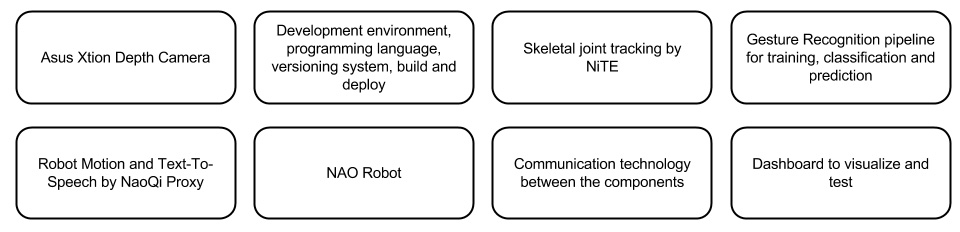
\includegraphics[height=35mm]{figures/content/hri-components.jpg} \caption{Component} \label{fg:hri:components} 
\end{figure}


\section{Experimental Designs} 
\subsection{Everything On-Board} First experiment design is conceived in a way that depth camera, skeletal joint tracking, gesture recognition infrastructure and robot motion will be embedded into the on-board computer of NAO. However, gesture recognition infrastructure is composed of computationally intensive machine learning processes and along with skeletal joint tracking by NiTE had pushed NAO to full CPU load consistently \cite{17}.

\subsection{Extending NAO with Single Board Computer} In order to escape the computational limitation of NAO, another experimental design was contemplated that the robot will be extended as shown in the figure \ref{fg:nao:bag} with a powerful Single Board Computer such as pcDuino or RaspberryPi. However, Asus Xtions higher power consumption of 2.5 Watts with weight of 250 grams, pcDuinos power consumption of 2A at 5VDC with weight of 100 grams and additional weight by 3D printed mounts, heat sinks and wires will make NAO to be heavier and ultimately result in poor motion performances and higher power consumption. 

\begin{figure}
	[h] \centering 
	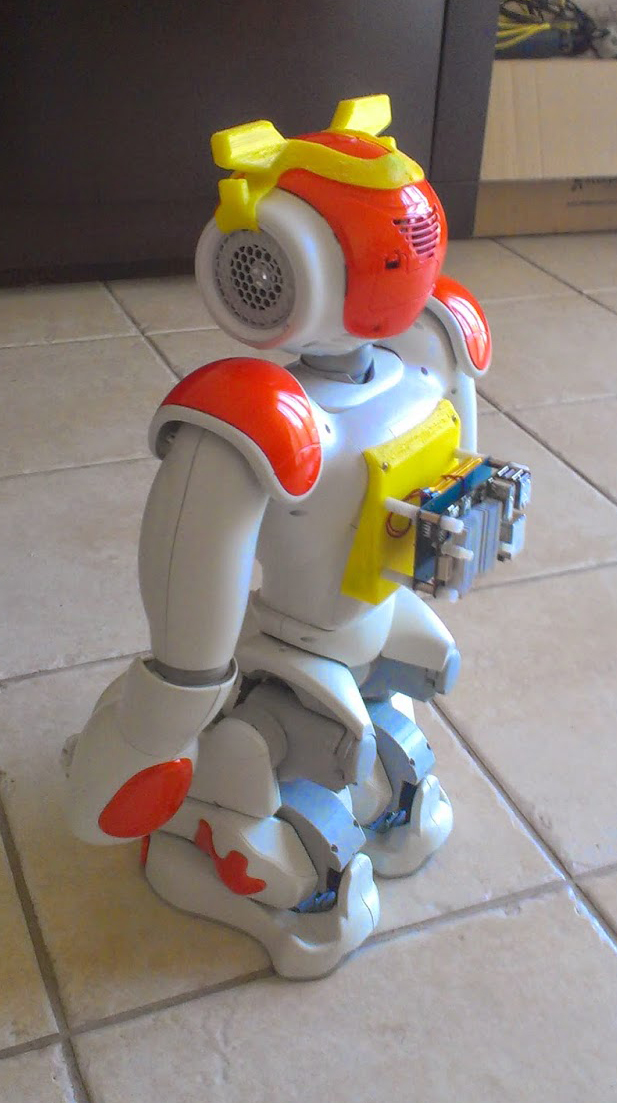
\includegraphics[height=7cm]{figures/content/nao-bag.jpg} \caption{3D printed mount to extend NAO with an external Single Board Computer. \cite{19} } \label{fg:nao:bag} 
\end{figure}


\subsection{Everything Off-Board} This experimental design pushes all the components to an off-board computer that could be a PC connected with depth camera at a fixed location. User will gesticulate in front of the camera and all processing will be done on PC. Finally predicted gesture will be transformed into a motion and voice, and it will be sent to NAO via Aldebaran proxies using WLAN. This design completely decouples the robot from other components and degrades the natural interaction between human and the robot. However, this design will suit for other applications such as indoor navigation and localization of NAO \cite{20}.

\section{Implementation} \label{sec:sol:impl} After analyzing the disadvantages of other experimental designs, the final design was chosen to build an efficient real-time hand gesture recognition for human-robot interaction using skeletal points. Figure \ref{fg:hri:architecture} shows the architecture of the solution that was implemented during this thesis by grouping many components into 4 different modules which serve several purposes. Each module is implemented in different environment as shown in the figure and they communicate with one another to complete the data flow. All these modules use a common configuration file named as \textit{hri.json} that contains information such as port number, host name and log path.

\begin{figure}
	[h] \centering 
	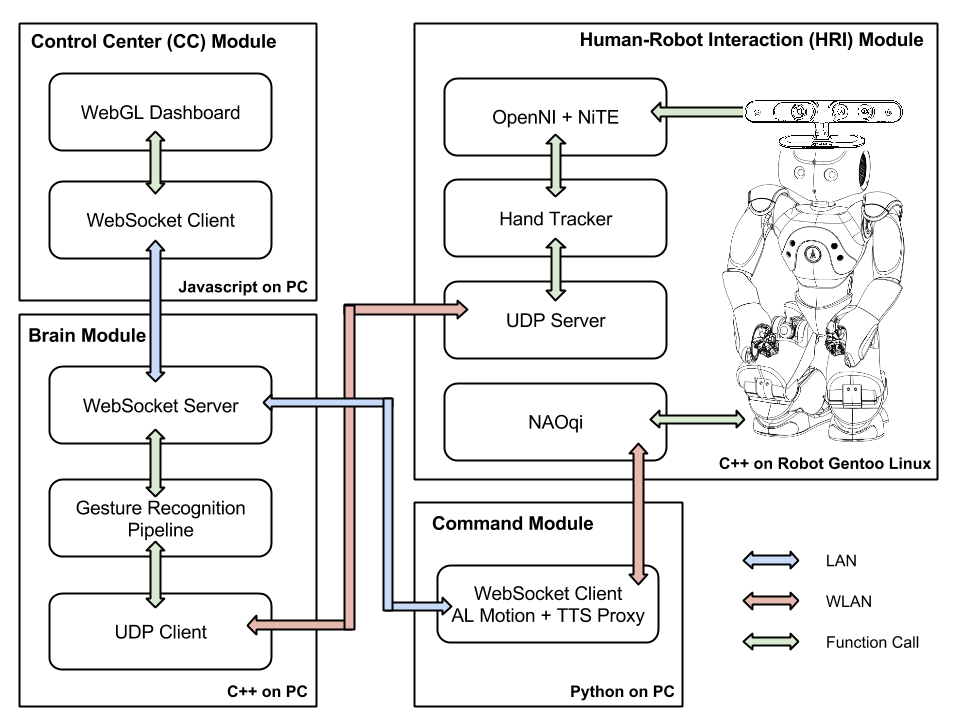
\includegraphics[height=11cm]{figures/content/hri-architecture.png} \caption{HRI Architecture} \label{fg:hri:architecture} 
\end{figure}


% Subsections of implmentation
\subsection{Human-Robot Interaction (HRI) Module} HRI module is implemented first to get the raw data from the depth sensor and process it to track the skeletal joint positions in real world coordinates. It is developed in C++ using a core library called Boost and NiTE 2 framework is used for the purpose of skeletal joints tracking. This module is deployed on the general purpose computer that is running inside the robot with necessary libraries and drivers.

Boost is a set of libraries for the C++ programming language that provide support for tasks and structures such as linear algebra, pseudo random number generation, multi threading, image processing, regular expressions, and unit testing. It contains over eighty individual libraries.

HRI module is composed of 3 components which are UDP Server, Gesture and Skeleton tracker. Flowchart \ref{fg:hri:flow} shows the data and control flow of this module where the user is asked to select Gesture or Skeleton tracker, when the program is started. It creates 2 threads depending on the selection: 
\begin{itemize}
	\item UDP Server thread - Asynchronously send data to the client and thread is always running. 
	\item Gesture or Skeleton tracker thread - A loop in the thread polls for a new frame from the depth camera till some key is pressed. If loop is interrupted, then the thread is exited and finally program is closed. 
\end{itemize}

Gesture and Skeleton tracker serve the purpose in extracting features from the raw data to implement a hand gesture recognition system. However, Skeleton tracker tracks 15 skeletal points in the human body and that leads to very intensive computation. Due to processing limitations of NAO, we chose to use Gesture tracker as it tracks only hand joints. Following sections describe internal working of HRI module.

\begin{figure}
	[h] \centering 
	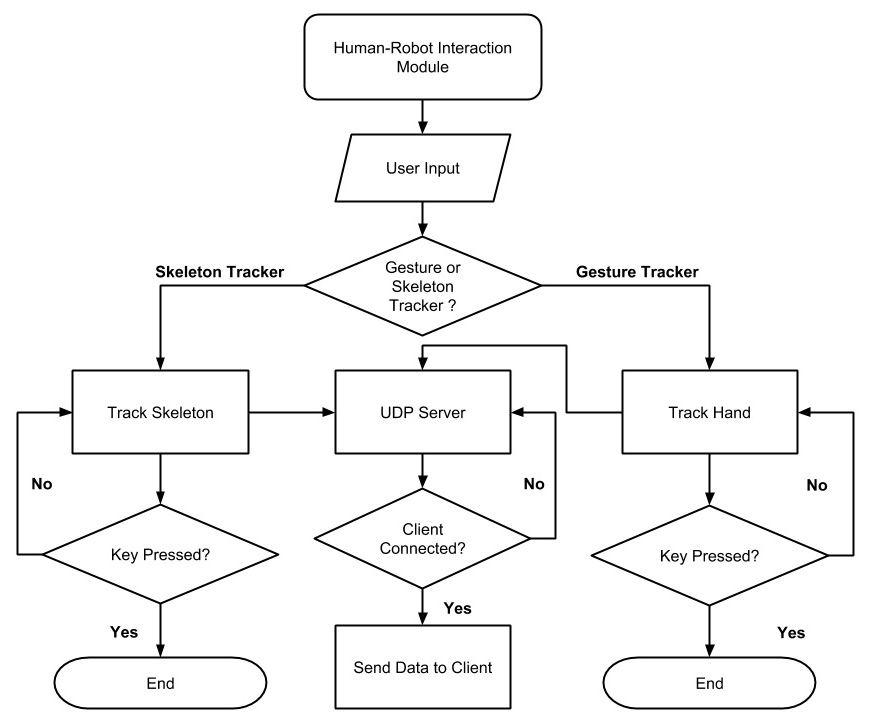
\includegraphics[height=115mm]{figures/content/hri-flow.jpg} \caption{HRI Module Control Flow} \label{fg:hri:flow} 
\end{figure}


\subsubsection{UDP Server} HRI module has to process the raw information from the depth camera and it has to send it to Brain module for the purpose of gesture recognition. As show in the architecture diagram \ref{fg:hri:architecture}, Brain module must be connected via Wireless Local Area Network (WLAN). WLAN at 2.4GHz readily is available on NAO and lead us to a solution, where we have to choose an UDP protocol to transmit the processed data from depth camera. UDP is chosen over other protocols because depth camera produces 30 depth images per second and transferring such a large amount of data using conventional communication technologies such as TCP will be create much overhead and delay in the communication.

Due to asynchronous requirement of the server, Boost Asio library is used to implement UDP server. Boost.Asio is a cross-platform C++ library for network and low-level I/O programming that provides developers with a consistent asynchronous model using a modern C++ approach.

UDP Server is basically an asynchronous programs that creates an UDP socket and listens to an port on the local machine. In this case, we have created a common configuration file named as \textit{hri.json} that contains port numbers for each module in this project. Therefore, this server listens to the 5005 on NAO and waiting for the clients to connect. 

Once the client is connected, it stores the endpoint details of the client such as IP address and the port number of the UDP client (Brain module), so that it can communicate with the Brain module whenever there is some data to be transmitted. Asynchronous functionality Boost.Asio calls the callback handler only when there is communication with the clients and waits in the thread for the next communication.

\subsubsection{Gesture Tracker} \label{sec:hri:ges} Gesture tracker is a component of HRI module that makes use of NiTE framework to localize the hand of the user in the field of view and track the hand position till the hand leaves the field of view (FOV) or hand is touching another object or hidden by an object. 

It uses \textit{HandTracker} class of NiTE framework and it needs to go through following steps before it can track a hand. Section \ref{sec:nite} discusses extensively about the functionalities of NiTE framework. 
\begin{itemize}
	\item NiTE framework must be initialized using \textit{nite::initialize()} function. 
	\item Depth camera must be connected and \textit{nite::HandTracker} must be created using OpenNI compatible device id. If not, default depth camera will be selected. 
	\item NiTE focus gesture WAVE must be initiated to localize the hand at first. 
	\item \textit{nite::HandTrackerFrameRef} must be read continuously for a new gesture. 
	\item If WAVE gesture is detected, then hand tracking will be started using the position of hand that triggered the gesture. 
\end{itemize}

Once the hand is been tracked, the hand will be added an id and it will be added to \textit{HandTrackerFrameRef}. NiTE framework allow users to add many number of hands and it will be tracked till there is enough computation power and hands are not overlapping. \textit{HandTrackerFrameRef} contains the array of all active hands and every hand is an object of \textit{nite::HandData}. It contains the position of the hand in 3 dimensional float stored in a class called \textit{Point3f}.

Unlike \textit{nite::UserTracker}, \textit{HandTracker} class can return only the hand position in the space and it can not specify whether it is a left or right hand. It is very necessary information for hand gesture training and classification because confused hand names will lead to a false model of the hand gesture and ultimately resulting in a bad performance. Hence, we have implemented a simple logic with the help of an assumption that user will gesticulate the focus gesture only in the order of right hand first and left hand second. 

However, functionalities gesture tracker are not only to track hand, but also send these information to Brain module via UDP. Therefore, C++ \textit{nite::HandData} objects must be serialized before transmitted over the network. Therefore, we chose JSON serialization and send them across the network as strings as shown in \ref{code:hand:data} 
\begin{lstlisting}
	{ "RIGHT": ["275.456", "339.026", "1841.850"], "LEFT": ["-456.289", "353.880", "1761.360"] } 
\end{lstlisting}
\label{code:hand:data}

Furthermore, HRI module send informations such as detected focus gesture and info messages to Brain module as shown in \ref{code:hand:info} to be displayed on the control center dashboard. Info messages helps us to know the status of the hand tracking algorithm which is the core component of HRI module. 
\begin{lstlisting}
	{"GESTURE":"WAVE"} {"GESTURE":"CLICK"} {"INFO": "Found new hand with id 1"} {"INFO": "LEFT Hand is lost"} {"INFO": "RIGHT Hand is lost"} {"INFO": "Both hands are lost"} {"INFO": "LEFT Hand is at FOV"} 
\end{lstlisting}
\label{code:hand:info}

\subsubsection{Skeleton Tracker} Skeleton Tracker is a component of HRI module that is more complex and computational intensive, since it uses \textit{nite::UserTracker} to track 15 bone joints of human body. Like Gesture Tracker in the section \ref{sec:hri:ges}, this component has to follow few procedure before tracking and it starts with an UDP server to unicast joint positions to Brain module. 
\begin{itemize}
	\item NiTE framework must be initialized using \textit{nite::initialize()} function. 
	\item Depth camera must be connected and \textit{nite::UserTracker} must be created using OpenNI compatible device id. If not, default depth camera will be selected. 
	\item Pose in front the camera as shown in the figure \ref{fg:ni:skeleton} to let the algorithm calibrate the body position. 
	\item \textit{nite::UserTrackerFrameRef }must be read continuously for a new user and if a new user is found, skeleton tracking will be started. 
\end{itemize}

\begin{figure}
	[h] \centering 
	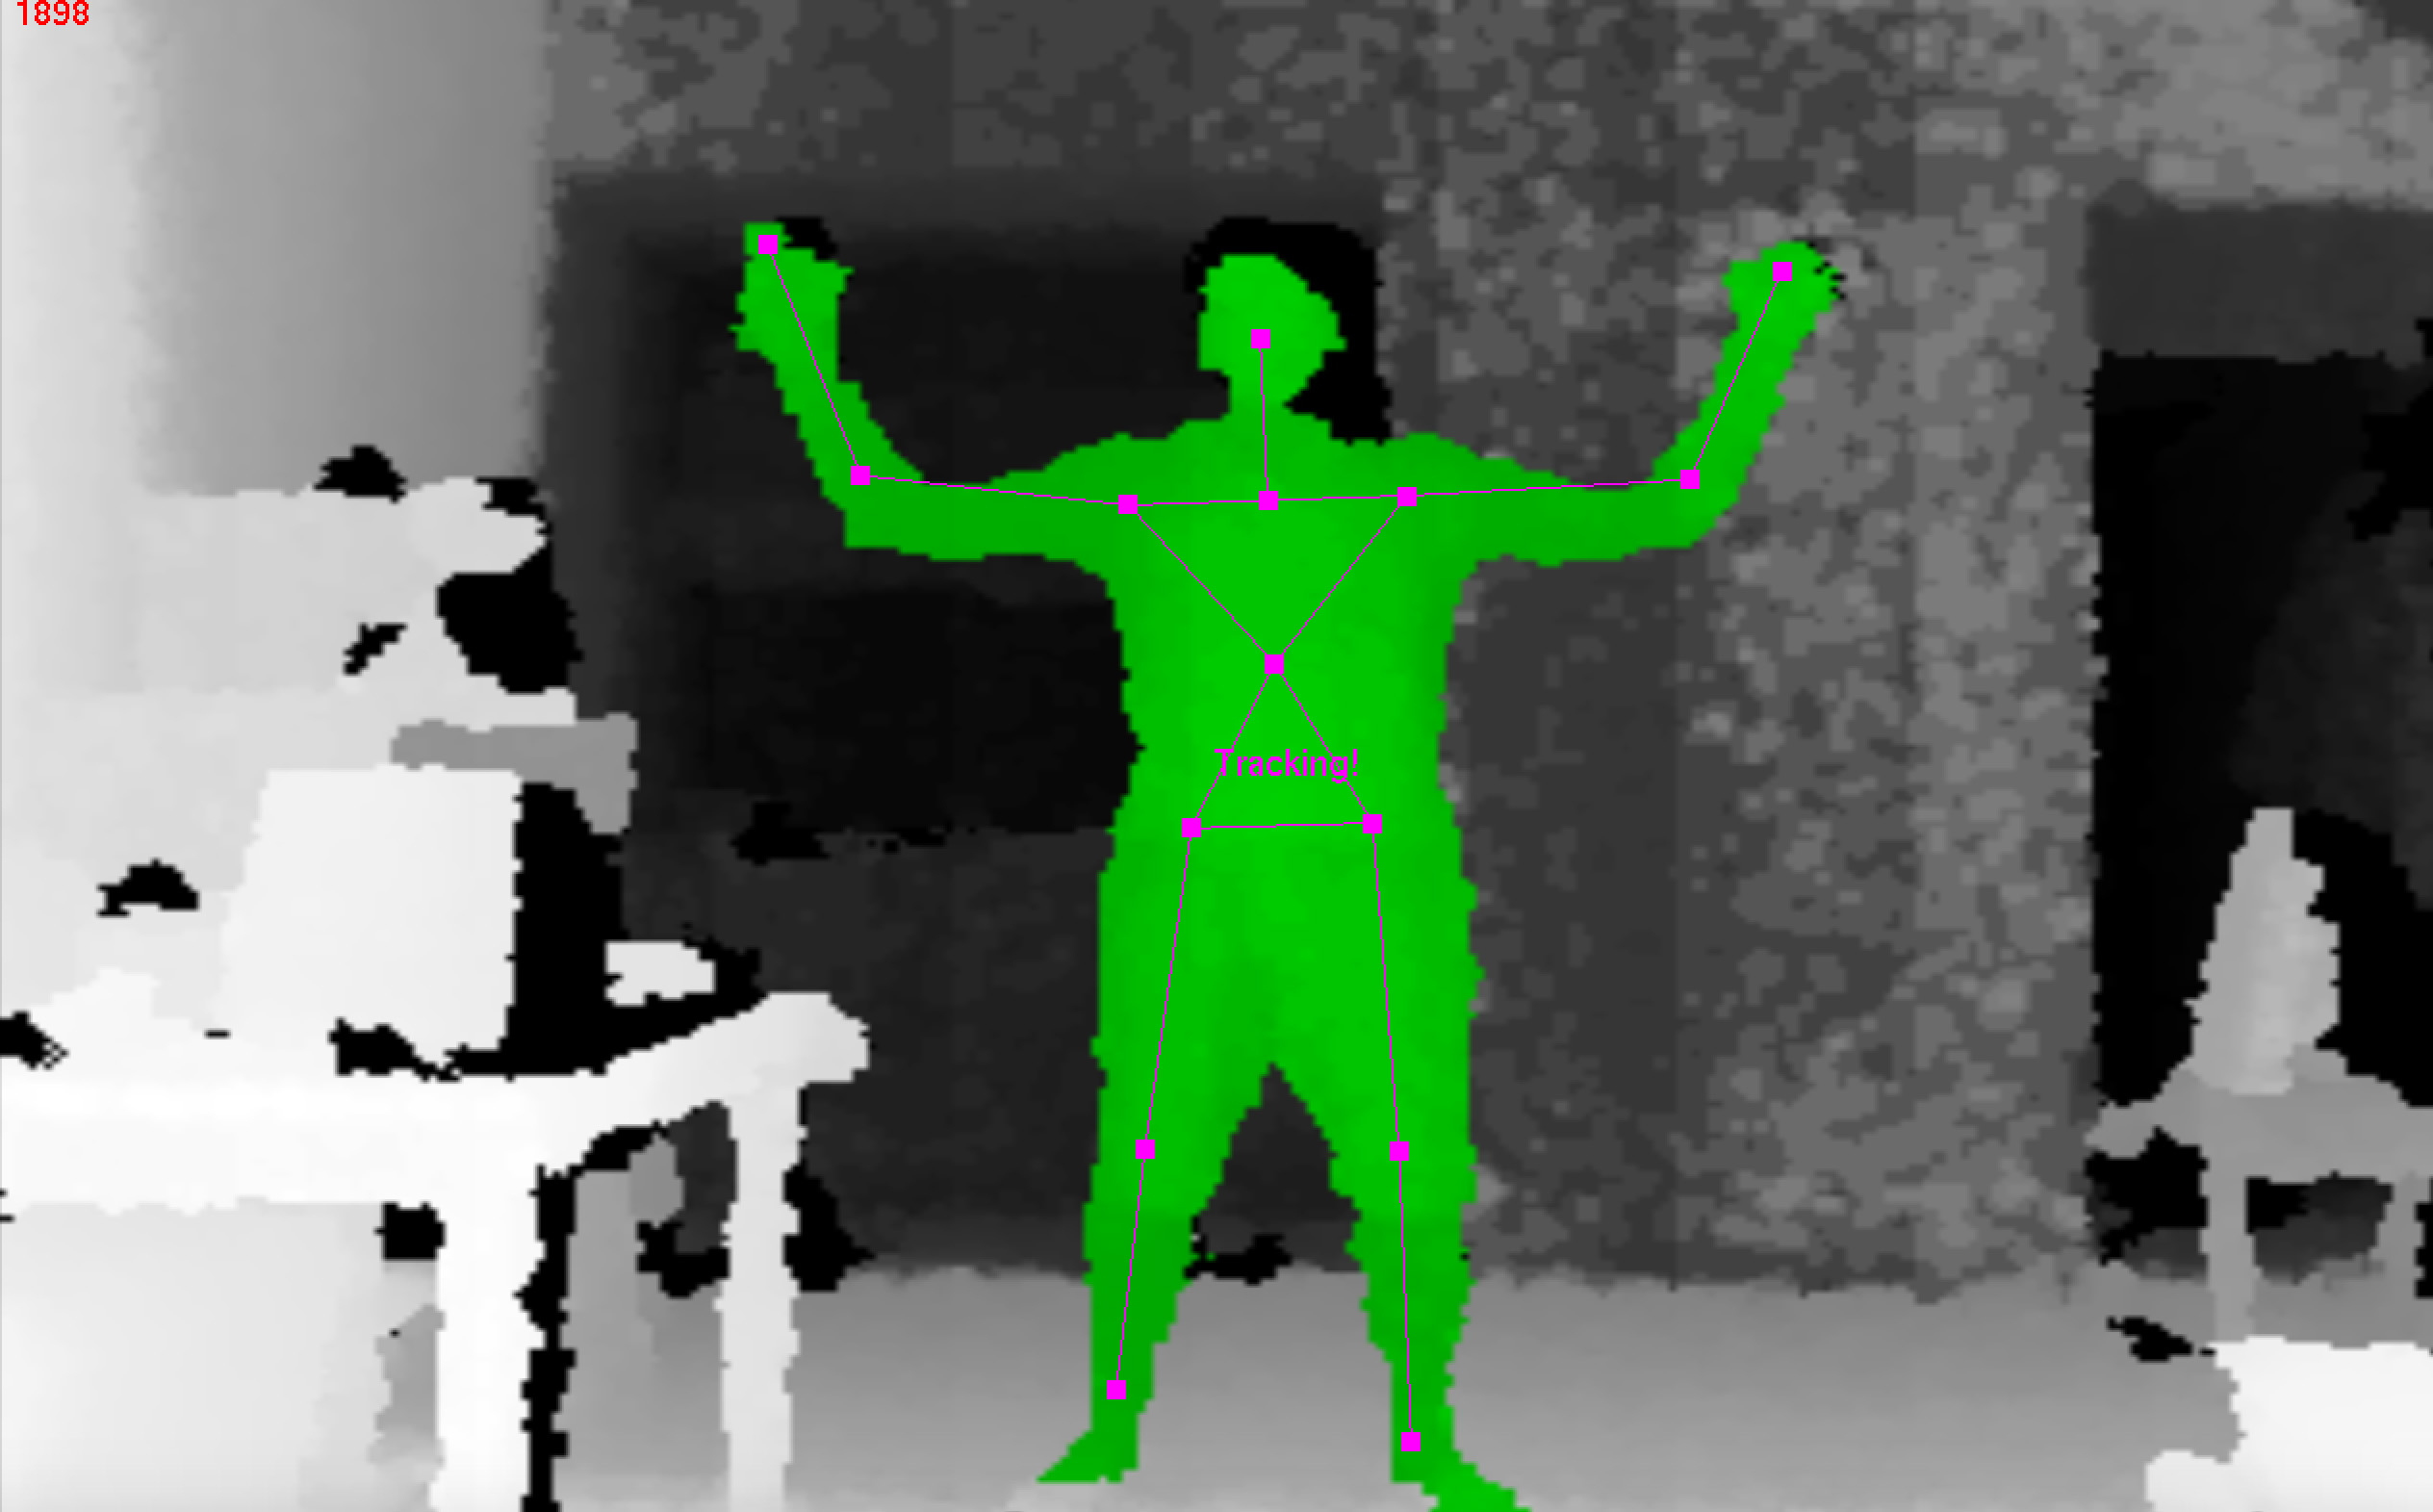
\includegraphics[width=145mm]{figures/content/ni-skeleton.jpg} \caption{Image captured while NiTE tracks 15 skeletal joints of the user using depth camera Asus Xtion. } \label{fg:ni:skeleton} 
\end{figure}


Unlike \textit{nite::HandTracker}, \textit{UserTracker} class of NiTE uses complex algorithms to keep tracking the skeleton even when the user poses in many ways. Therefore, it needs the data provided by NiTE framework which contain models of 1 million training samples. In addition, \textit{UserTracker} can return 15 skeletal joints position and orientation and they are labeled by the joint name. This feature helps us to avoid the implementation to find the hand name. Moreover, details of joint orientations offer us a chance to calculate positions not only in Cartesian coordinates, but also in spherical coordinates system which is essential for many complex hand gesture recognition solutions \cite{21}. Furthermore, \textit{SkeletonJoint} class indicates how sure the NiTE skeleton algorithm is about the joint position. The value is between 0 and 1, with increasing value indicating increasing confidence. Section \ref{sec:nite} discusses extensively about the algorithm of NiTE.

Finally, Skeleton tracker serializes the C++ \textit{nite::UserData} objects to JSON and sends asynchronously to the client for further gesture recognition procedures. 

%\subsection{Brain Module} Brain module is the core functional part of this thesis. It is named as Brain since it refers to the anatomical brain that plays the vital role of the human life in learning, classifying, predicting and decision making. 

Brain module is composed of 3 components which are UDP Client, Brain (Gesture Recognition Pipeline) and WebSocket Server. Flowchart \ref{fg:brain:flow} shows the data flow of this module where the user is asked to select Prediction or Training of Hand Viewer mode, when the program is started. It creates a thread and runs a loop on the main thread depending on the selection: 

\begin{itemize}
	\item UDP Client thread - Asynchronously receiving data from HRI module and thread is always running.
	\item Prediction or Training of Hand Viewer on main program thread -  Loop in the main thread run always and check if the Brain module is in prediction or training mode. If loop is interrupted, then the thread is exited and finally program is closed.	
\end{itemize}

\begin{figure}
	[h] \centering 
	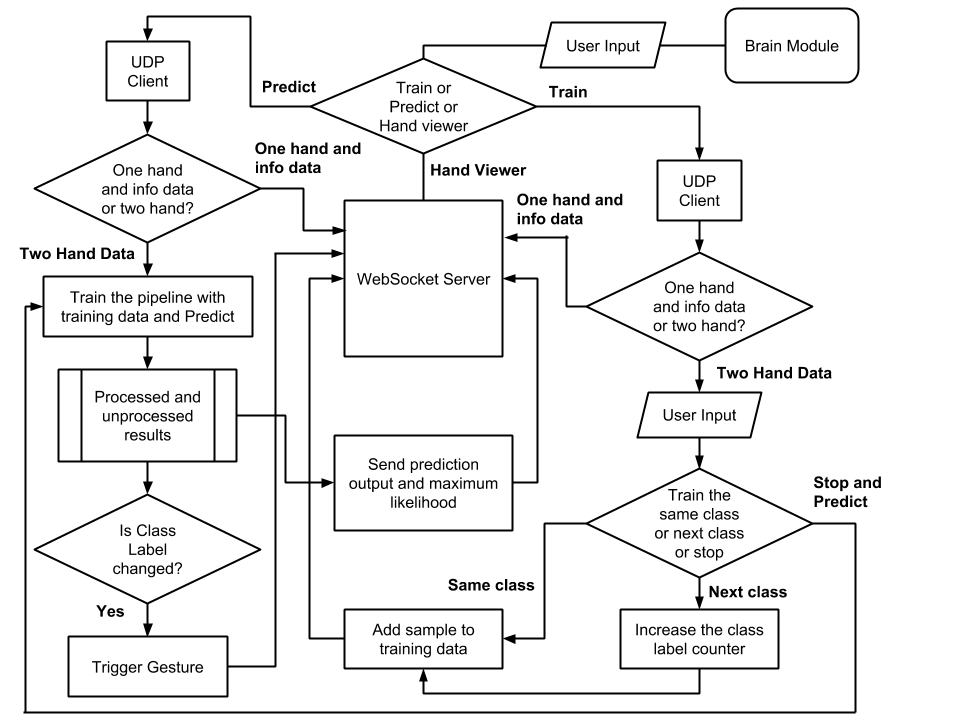
\includegraphics[height=115mm]{figures/content/brain-flow.png} \caption{Brain Module Control Flow} \label{fg:brain:flow} 
\end{figure}


\subsubsection{UDP Client}
Brain module receives processed information such as joint positions, detection of focus gestures and info messages from the HRI module as UDP stream of JSON strings via WLAN. Like the UDP Server built inside HRI module, this is also an asynchronous socket that starts at port 5006 and connects to the server by resolving the serverHostName and port number from the common configuration file. Once it is connected, it receives the data from HRI module, when it is started tracking a hand or skeleton and asynchronously calls the callback handler.

Since data is transmitted as JSON strings, it has to be parsed and relevant informations must be extracted. For this purpose RapidJSON parser is used. Data flow of Brain module is mainly handled in the callback handler of UDP client because it acts as a source of input. Whenever there is a new data arrived, this asynchronous callback handler is called and it does the following tasks as shown in the flowchart \ref{fg:brain:flow} :

\begin{itemize}
	\item Extract only newly received data from the buffer by trimming the JSON
	\item Parse the trimmed JSON to populate hand data vectors. 
	\item If focus gesture or info messages or only one hand data is received, send it via WebSocket to the clients
	\item Check if the module is Prediction or Training or Hand Viewer mode
	\item In the prediction mode :
		\begin{itemize}
		\item If the positions of both hands are received, predict the class label
		\item Add predicted class label and maximum likelihood to the sample, and send it via WebSocket
		\item If there is a class label not than 0, then send the respective gesture name via WebSocket
		\end{itemize}
	\item If it is in the training mode and both hands are received, then add them to the training data
	\item If it is in the hand viewer mode, just forward all the data to the clients via WebSocket
\end{itemize} 

\subsubsection{Brain}
This is the core component of Brain module that plays a vital role in training, classifying and predicting the hand gestures. As described in the section \ref{sec:grt}, this component is based on the gesture recognition pipeline provided by Gesture Recognition Toolkit (GRT).

Flowchart \ref{fg:brain:flow} shows various tasks involved in training and predicting phase of this module. However, GRT pipeline must be configured and customized in order to be a productive gesture recognition system.

\paragraph*{Classifier} Adaptive Naive Bayes Classifier (ANBC) is chosen to be used in this thesis as described in the section \ref{sec:anbc}. Training data for the same gesture will vary in range from person to person and position to position. Therefore the classifier is enabled for Min-Max scaling that is basically a normalization by rescaling the values between 0 to 1.  This is done by calling enableScaling(true) function of the classifier.

\paragraph*{Null Rejection} Enabling the scaling with ANBC will classify every input samples to belong to any of the class and thereby, do not have the ability to detect non-gestures. In order to avoid this catastrophe GRT offers Null Rejection features to the algorithms, by this function enableNullRejection(true) and also provides a function to set how big the rejection region should be, by setNullRejectionCoeff(1).

\paragraph*{Post Processing} As discussed in the section \ref{sec:grt}, prediction output must be post processed in order to avoid false gesture spikes. Therefore, class label filter is added to the pipeline by with this function ClassLabelFilter(30,60). Minimum count is set to 30 with the buffer size of 60 for the reason that the user must gesticulate for minimum of one second and depth camera produces 30 frames per second. Additionally  ClassLabelChangeFilter() is added so that there is only one output of the predicted class label, when there is a change in the gesture and all other time it outputs 0, that is reserved for non-gesture.

\paragraph*{Training Data} We used ClassificationData data structure of GRT to collect training data of static gestures. It must be initialized with number of dimensions the samples will be. In our thesis we modeled hand gestures with two hand positions in 3 dimensional Cartesian coordinates, therefore training data has 6 dimensions.
As described in the section \ref{sec:grt}, GRT enables us to execute various operations on the training data such as recording, labeling, partitioning and testing.  

\paragraph*{Training} When Brain is set to training mode, it starts the TrainingDataRecordingTimer. We have configured 20 seconds recording time and 15 seconds preparation time. Preparation time helps the trainer to go in front of depth camera and stay in the pose of the gesture that is going to be recorded. Furthermore, It initializes the Class Label to 1 and it will be increased by one for other classes. Class Label can not be assigned to 0 because GRT reserves it for non-gestures. If positions of left and right hand are received from the HRI module, Brain starts to add the samples with the chosen Class Label to the training data till the timer is in recording mode and simultaneously it sends to received samples via WebSocket to the clients to visualize. When the recording timer is stopped, Brain requests the trainer to choose any of the following options :

\begin{itemize}
	\item Train the same class again - New samples will be added to the training data for same Class Label.
	\item Train the next class - Class Label is increased by one and new samples are added.
	\item Stop training and go to prediction mode - Saves the training data to a file named as hri-training-dataset.txt and trains the pipeline and goes into prediction mode
\end{itemize}

\paragraph*{Prediction} When Brain is set to prediction mode, first thing it does, is loading the training labeled classification data and train the pipeline to create models for each gesture. Second step is to look for any specific pipeline configuration such as classifier and pre/post processing modules. Such configurations can also be loaded into pipeline as GRT pipeline files. This feature of GRT offers us an opportunity to run the gesture recognition application using dynamic configurations. Once Brain starts to receive input samples via UDP, it feeds it to the pipeline to predict. Finally, the prediction results such as predicted class label, maximum likelihood, class distances and weights can returned by the pipeline. Flexible GRT pipeline provides many more features such as post-processed and unprocessed prediction results. Therefore, the prediction results for every input sample can be obtained. The post-processed result will allow Brain to send the detected gesture only once, even if the user is continuously gesticulating the same gesture.  

\subsubsection{WebSocket Server}
WebSocket class is developed using websocketpp C++ library that basically uses BOOST libraries. It is a simple implementation of WebSocket server that listens to the port number 5008. The port number can be configured dynamically by loading the common configuration file. WebSocket class is initialized by UDP Client class and keeps the server running in a separate thread. Once clients such as CC module and Command module are connected, it stores the endpoint connection handlers of them for later communication.  
%\subsection{Control Center (CC) Module} Control Center plays an important role in this thesis. It is the eye that visualizes the internal status of the modules. It was first built for the purpose of visually render the skeletal points of the human body that is being tracked by NiTE. Later, it became one place to interact with the whole system. 

CC is developed in Javascript with the help of WebGL and jQuery. The cloud computing is day by day pushing computer applications to the Internet, which allows softwares to be operated using internet-enabled devices. Due to this reason browser based cross-compatible applications are getting popular and that leads to the huge involvement of development in Javascript. Therefore, we chose a cross-compatible platform that work out of the box than implementing the same in C++ using OpenGL.

\begin{figure}
	[h] \centering 
	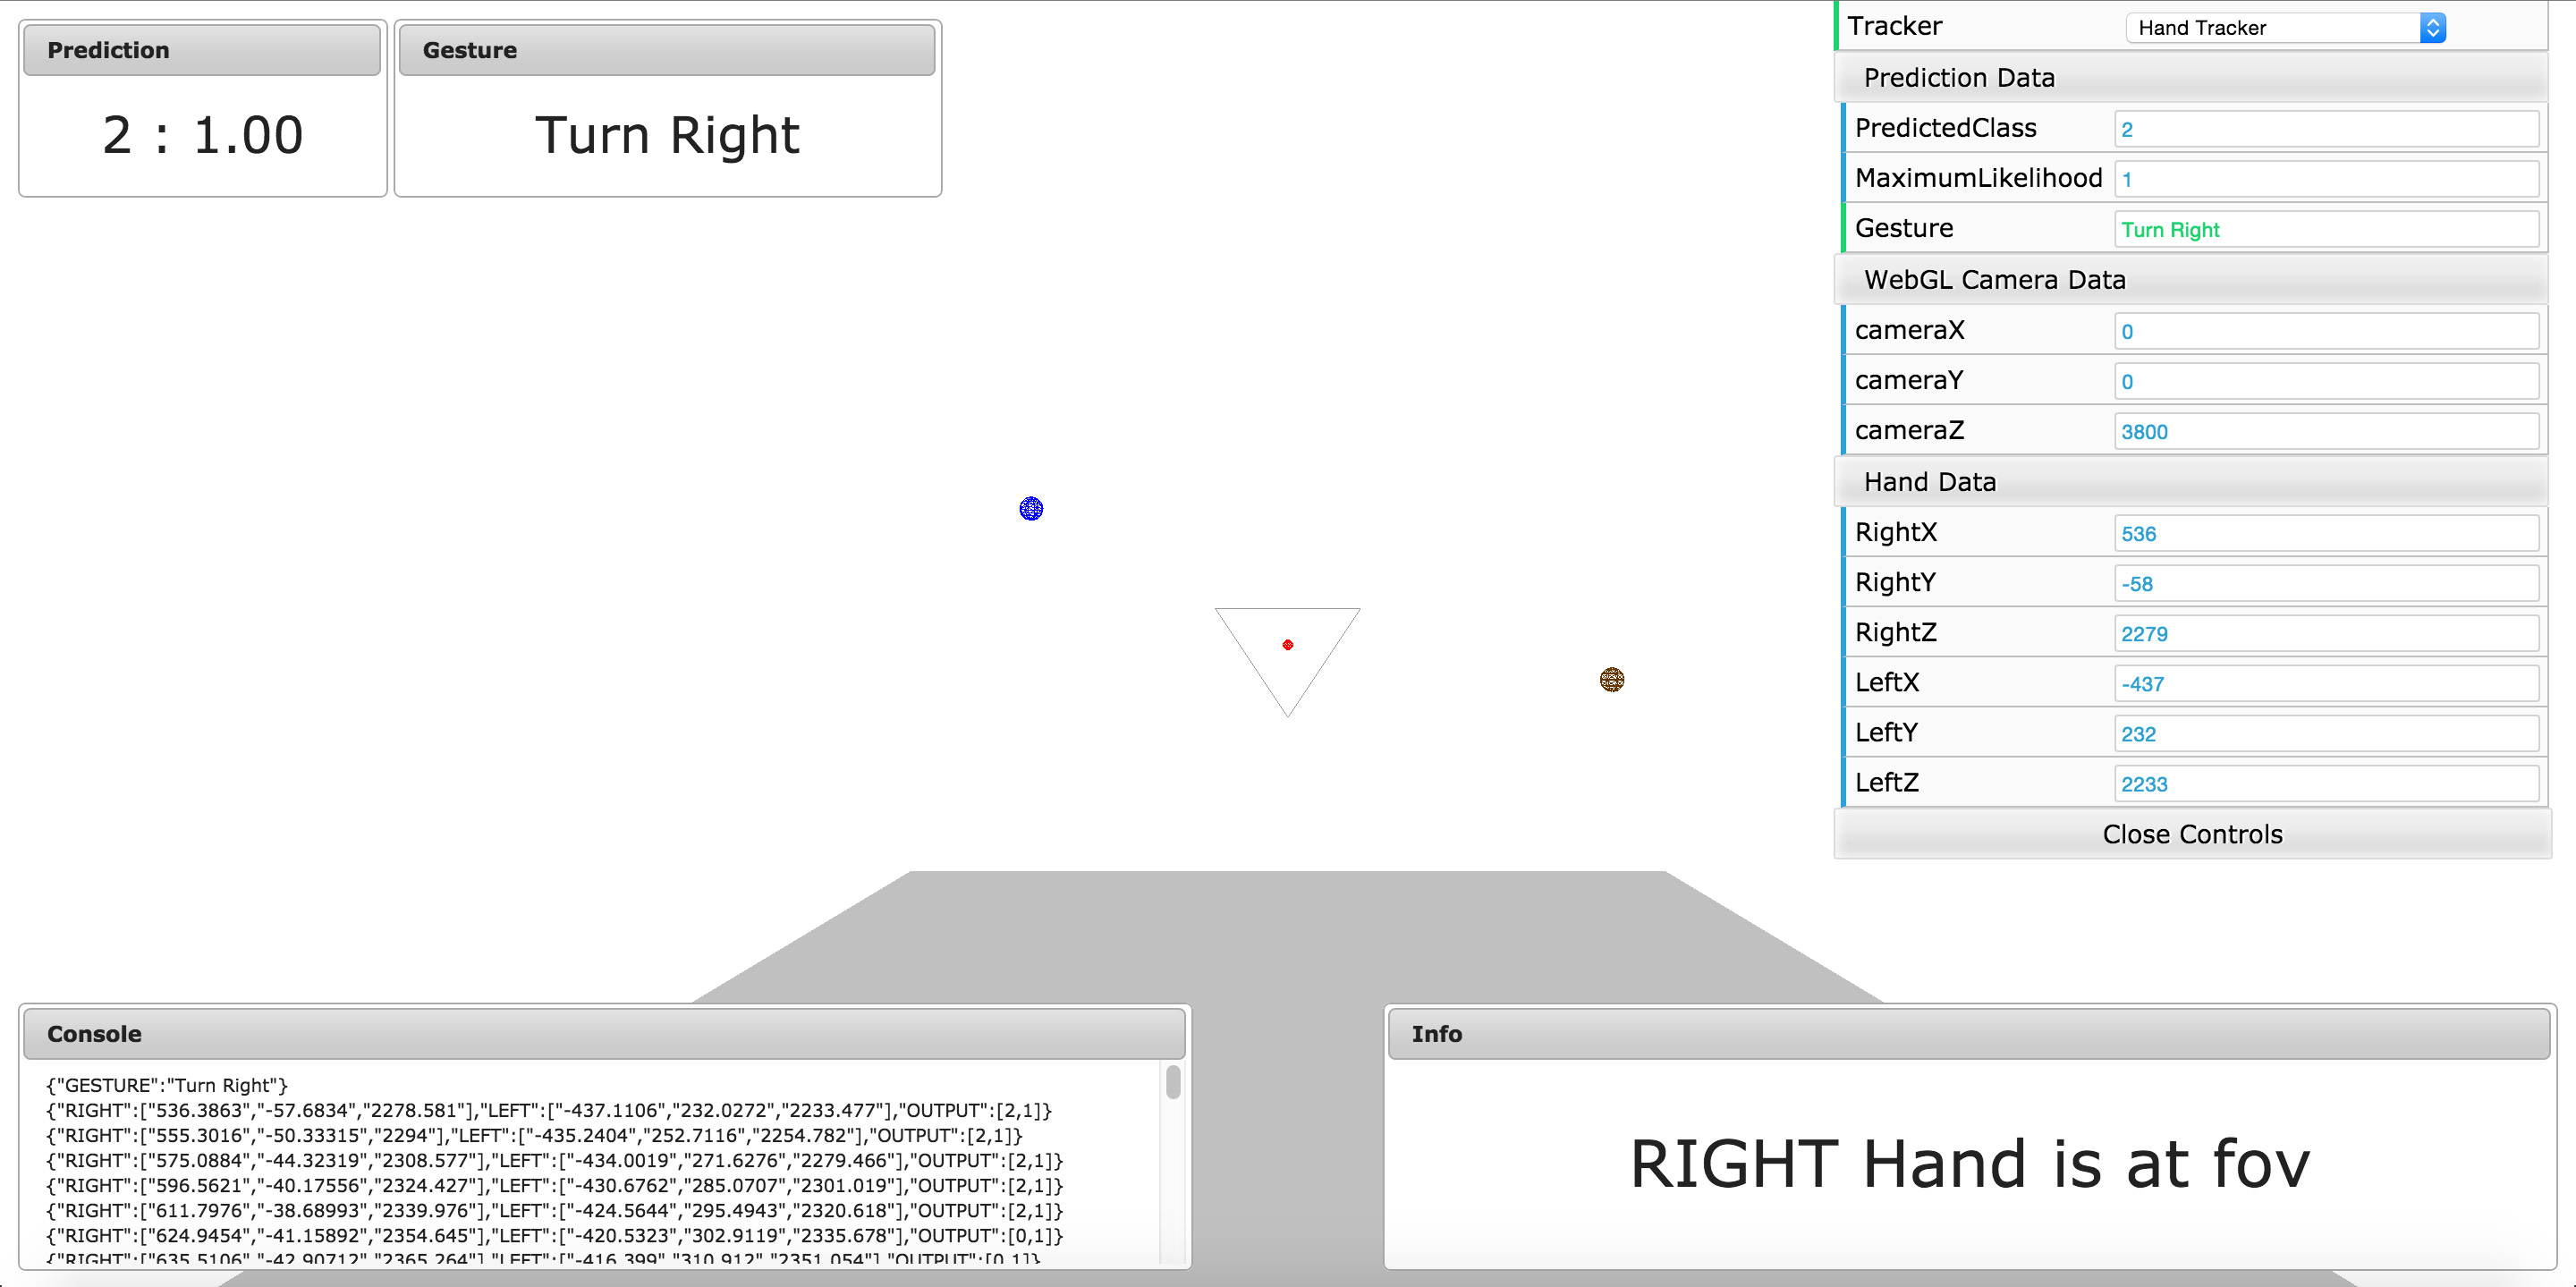
\includegraphics[width=120mm]{/content/cc-hand.jpg} \caption{Control Center displays received data of hand positions and prediction results} \label{fg:cc:hand} 
\end{figure}

\paragraph*{Javascript} It is a dynamic programming language whose implementations allow client-side scripts to interact with the user, control the browser, communicate asynchronously, and alter the document content that is displayed. However, It is also used in server-side network programming with runtime environments such as Node.js, game development and the creation of desktop and mobile applications.

\paragraph*{ThreeJS} It is a lightweight 3D library with a very low level of complexity, written purely in Javascript that can render 3D objects in various renderer such as canvas, svg, CSS3D and WebGL. In this thesis, we have chosen WebGL renderer to implement the Control Center since it is faster than others in rendering tracked skeletal points at 30 frames per second.

\paragraph*{WebSocket Client} CC receives the data from Brain modules via WebSocket. The client uses the native Javascript WebSocket implementation that is supported by many latest browsers. It connects to the WebSocket server that is listening on the port 5008. When the client receives the data, it updates the data buffer asynchronously.

\paragraph*{Architecture} Control Center is implemented in MV* (Model View) design pattern that is quite popular among Javascript developers. Since the requirement of this module needs many libraries, a dependency injection library called RequireJS is used to load all the libraries when the application is opened in the browser.  

\paragraph*{Libraries} Along with ThreeJS, libraries such as jQuery, underscore, TrackBallControl and datGUI are used in this module. jQuery is most common library for Document Object Model (DOM) manipulation in the browser. Operations on arrays and objects are made easier with the help of underscore. TrackBallControl allows to do manipulations such as rotate, revolve and transform the objects which rendered in WebGL. datGUI is a lightweight simple library to create GUI elements to build a dashboard in few lines of code.

\begin{figure}
	[h] \centering 
	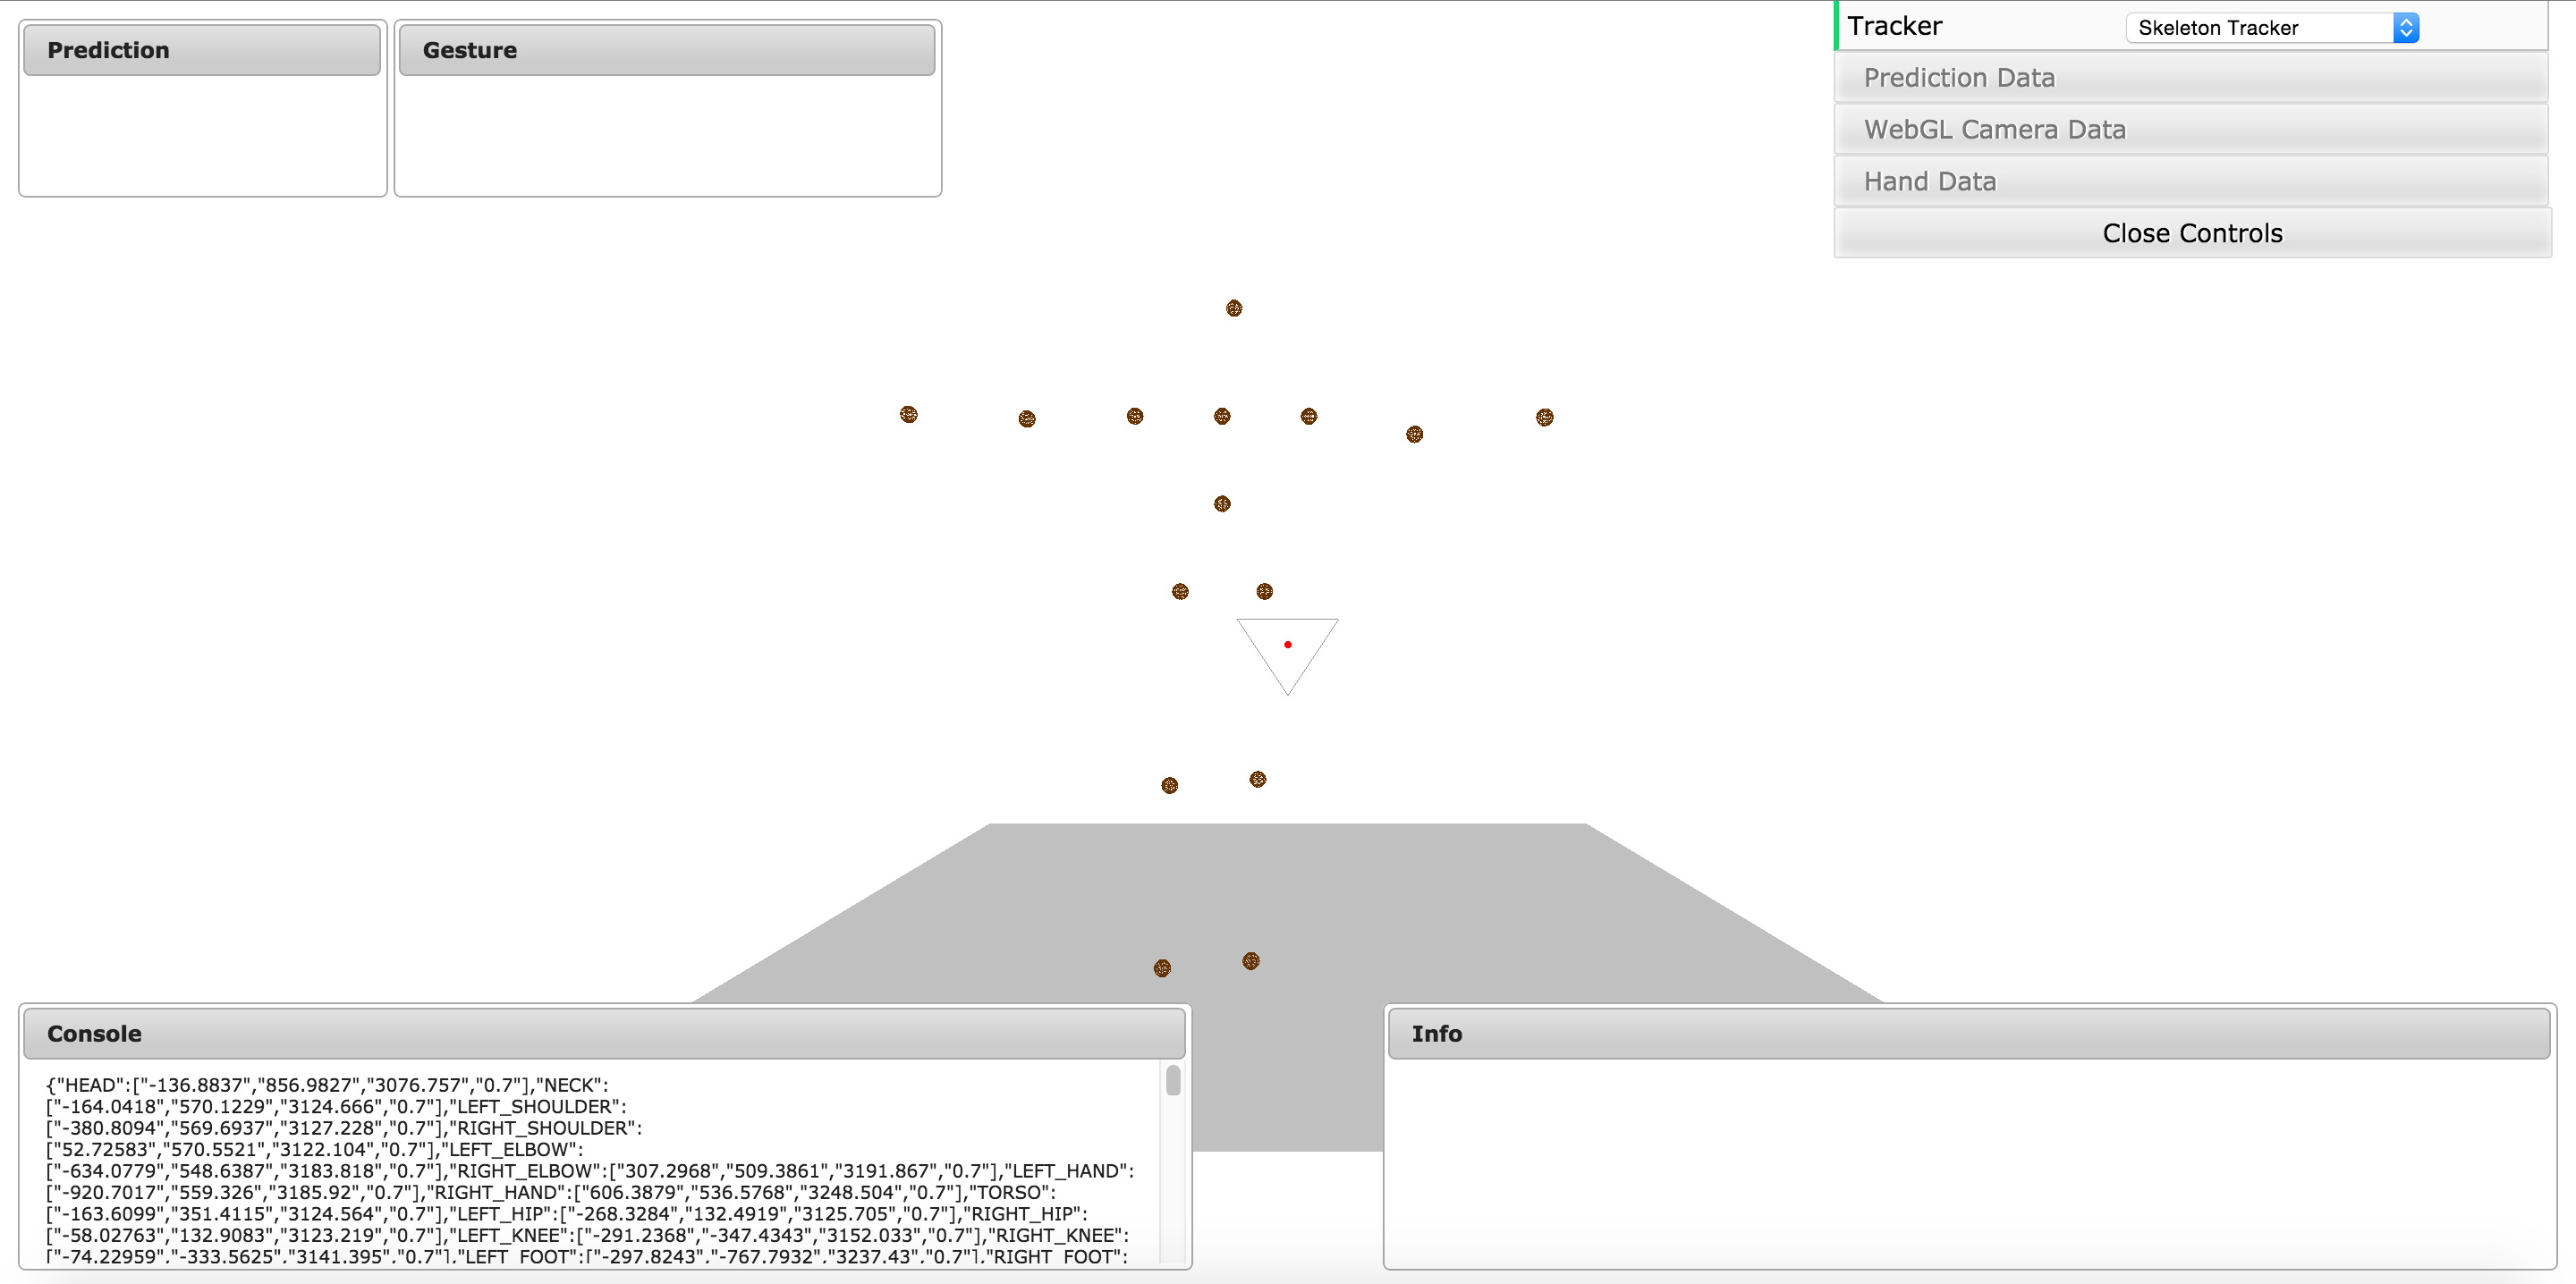
\includegraphics[width=145mm]{figures/content/cc-skeleton.jpg} 
	\caption{Control Center renders real time positions of 15 human skeleton joints.} 
	\label{fg:cc:skeleton} 
\end{figure}

\paragraph*{Model and View} To avoid complexity this Javascript application does not have any sophisticated model. It simply uses an array named skeletonBuffer that holds the JSON data received via WebSocket. All these actions are carried out in the store of the application. View does large part of the work for CC. At first it initializes the DOM and add GUI elements to it. Then ThreeJS scene is created with WebGL renderer and adds a perspective camera, a plane geometry as a base and a triangle to show origin of the sensor. By default CC is in hand tracking mode and it creates two spheres to visualize the position of left and right hand. In skeleton tracking mode it creates 15 spheres two show all the skeletal points that are being tracked by NiTE. Control Center offers us to replay the positions of joints by storing them to a file and selecting Hand Tracker From Data option in the GUI. View automatically iterates through all the objects in the array and renders them at 60 fps. 

\paragraph*{User Interface (UI) } Figure \ref{fg:cc:hand} the dashboard of the Control Center. Console box is an UI element that shows all the incoming data via WebSocket. It allows us to scroll through the data, if there is a necessity to cross check the data. Right bottom shows Info box which is created for the purpose of showing all intercommunication messages among all the modules. For example, "RIGHT Hand is at FOV" is an info message triggered by NiTE to inform that hand is closer to the field of view (FOV) and it may lose the hand. Left top corner displays two UI elements which are meant to show the prediction result for every input sample and recognized gesture  that is triggered only after gesticulating it for more than one second. Furthermore, top right corner of the dashboard reveals more internal variables such as WebGL camera positions and real time hand in 3 dimensional Cartesian coordinates. CC can not only render hand joints, but also complete human skeleton with 15 skeletal point which are being tracked as shown in the figure \ref{fg:cc:skeleton}. It also allows us to save tracking data to a json file and replay them by choosing appropriate mode from the drop down list on the top right corner.




%\subsection{Command Module} Last but not the least module to complete the functionalities of our hand gesture recognition system is the Command module. All other modules which are described above need the Command module to interact with the robot.

Command module is developed in Python with WebSocket and NAOqi libraries. Python is a widely used general-purpose, high-level programming language. Its design philosophy emphasizes code readability, and its syntax allows programmers to express concepts in fewer lines of code than would be possible in languages such as C++ or Java. 

Command modules initiates the WebSocket Client and it connects to the Brain modules WebSocket Server at a given port number by loading the common configuration file. WebSocket client keeps the main thread run forever and it executes the respective call back handlers. When there is a new message, it calls the \textit{onMessage} handler and parses the received JSON data to a python object. Whenever gesture data is received, it is translated to a robotic speech and motion via NAOqi proxies.

We have used ALMotions Locomotion Control extensively to move the robot from one position to another based on the recognized hand gesture such as "Turn Left" or "Move Right". Additionally, Gesture-To-Gesture actions where a human hand gesture is translated to the robot hand gesture by using the Joint Control of ALMotion module.

%\subsection{Head Mount} As described earlier in the section \ref{sec:nao:vision}, integrated hardwares of NAO Vision are not sufficient to provide precise three dimensional data to the complex algorithms to track human skeletal joints. Therefore, Asus Xtion PRO LIVE 3D camera is chosen to be used for this gesture recognition system. Section \ref{sec:sol:impl} shows the final architecture that proposes to mount Asus Xtion on the head of the robot. 

\begin{figure}	 	
	\begin{minipage}
		{.45 
			\textwidth} 
		\centering 
		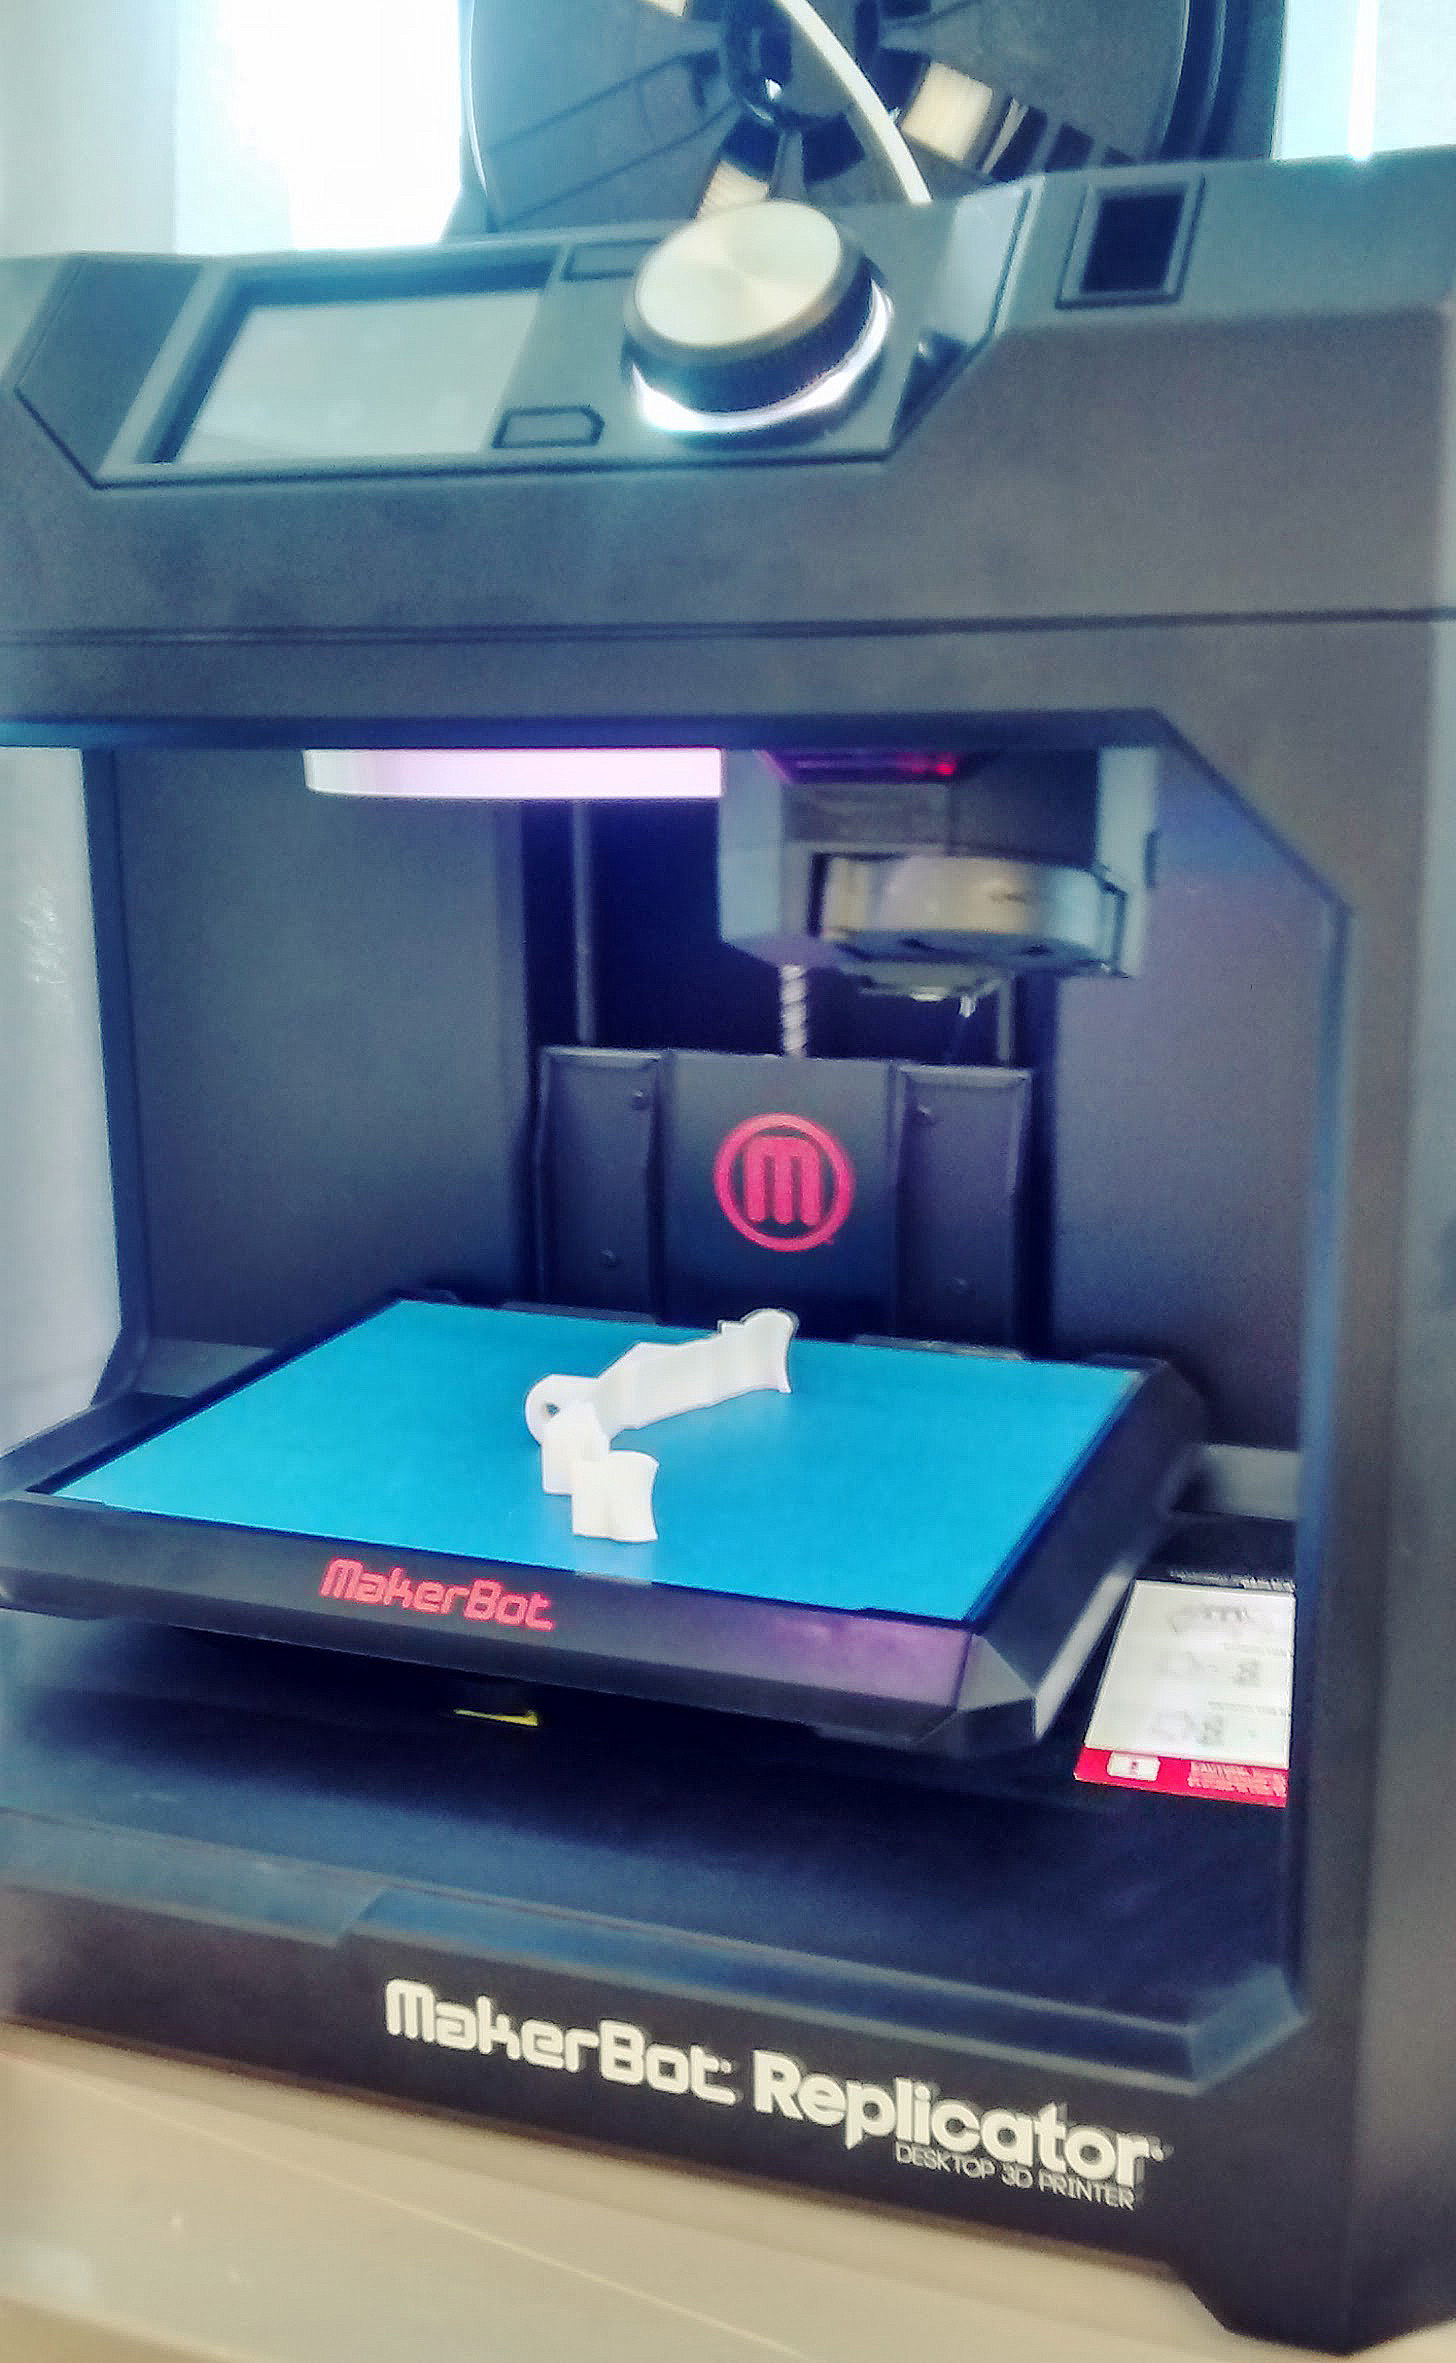
\includegraphics[height=60mm]{figures/content/xtion-mount-3d.jpg} \caption*{3D printing the mount} 
	\end{minipage}
	\begin{minipage}
		{.45 
			\textwidth}  
		\centering
		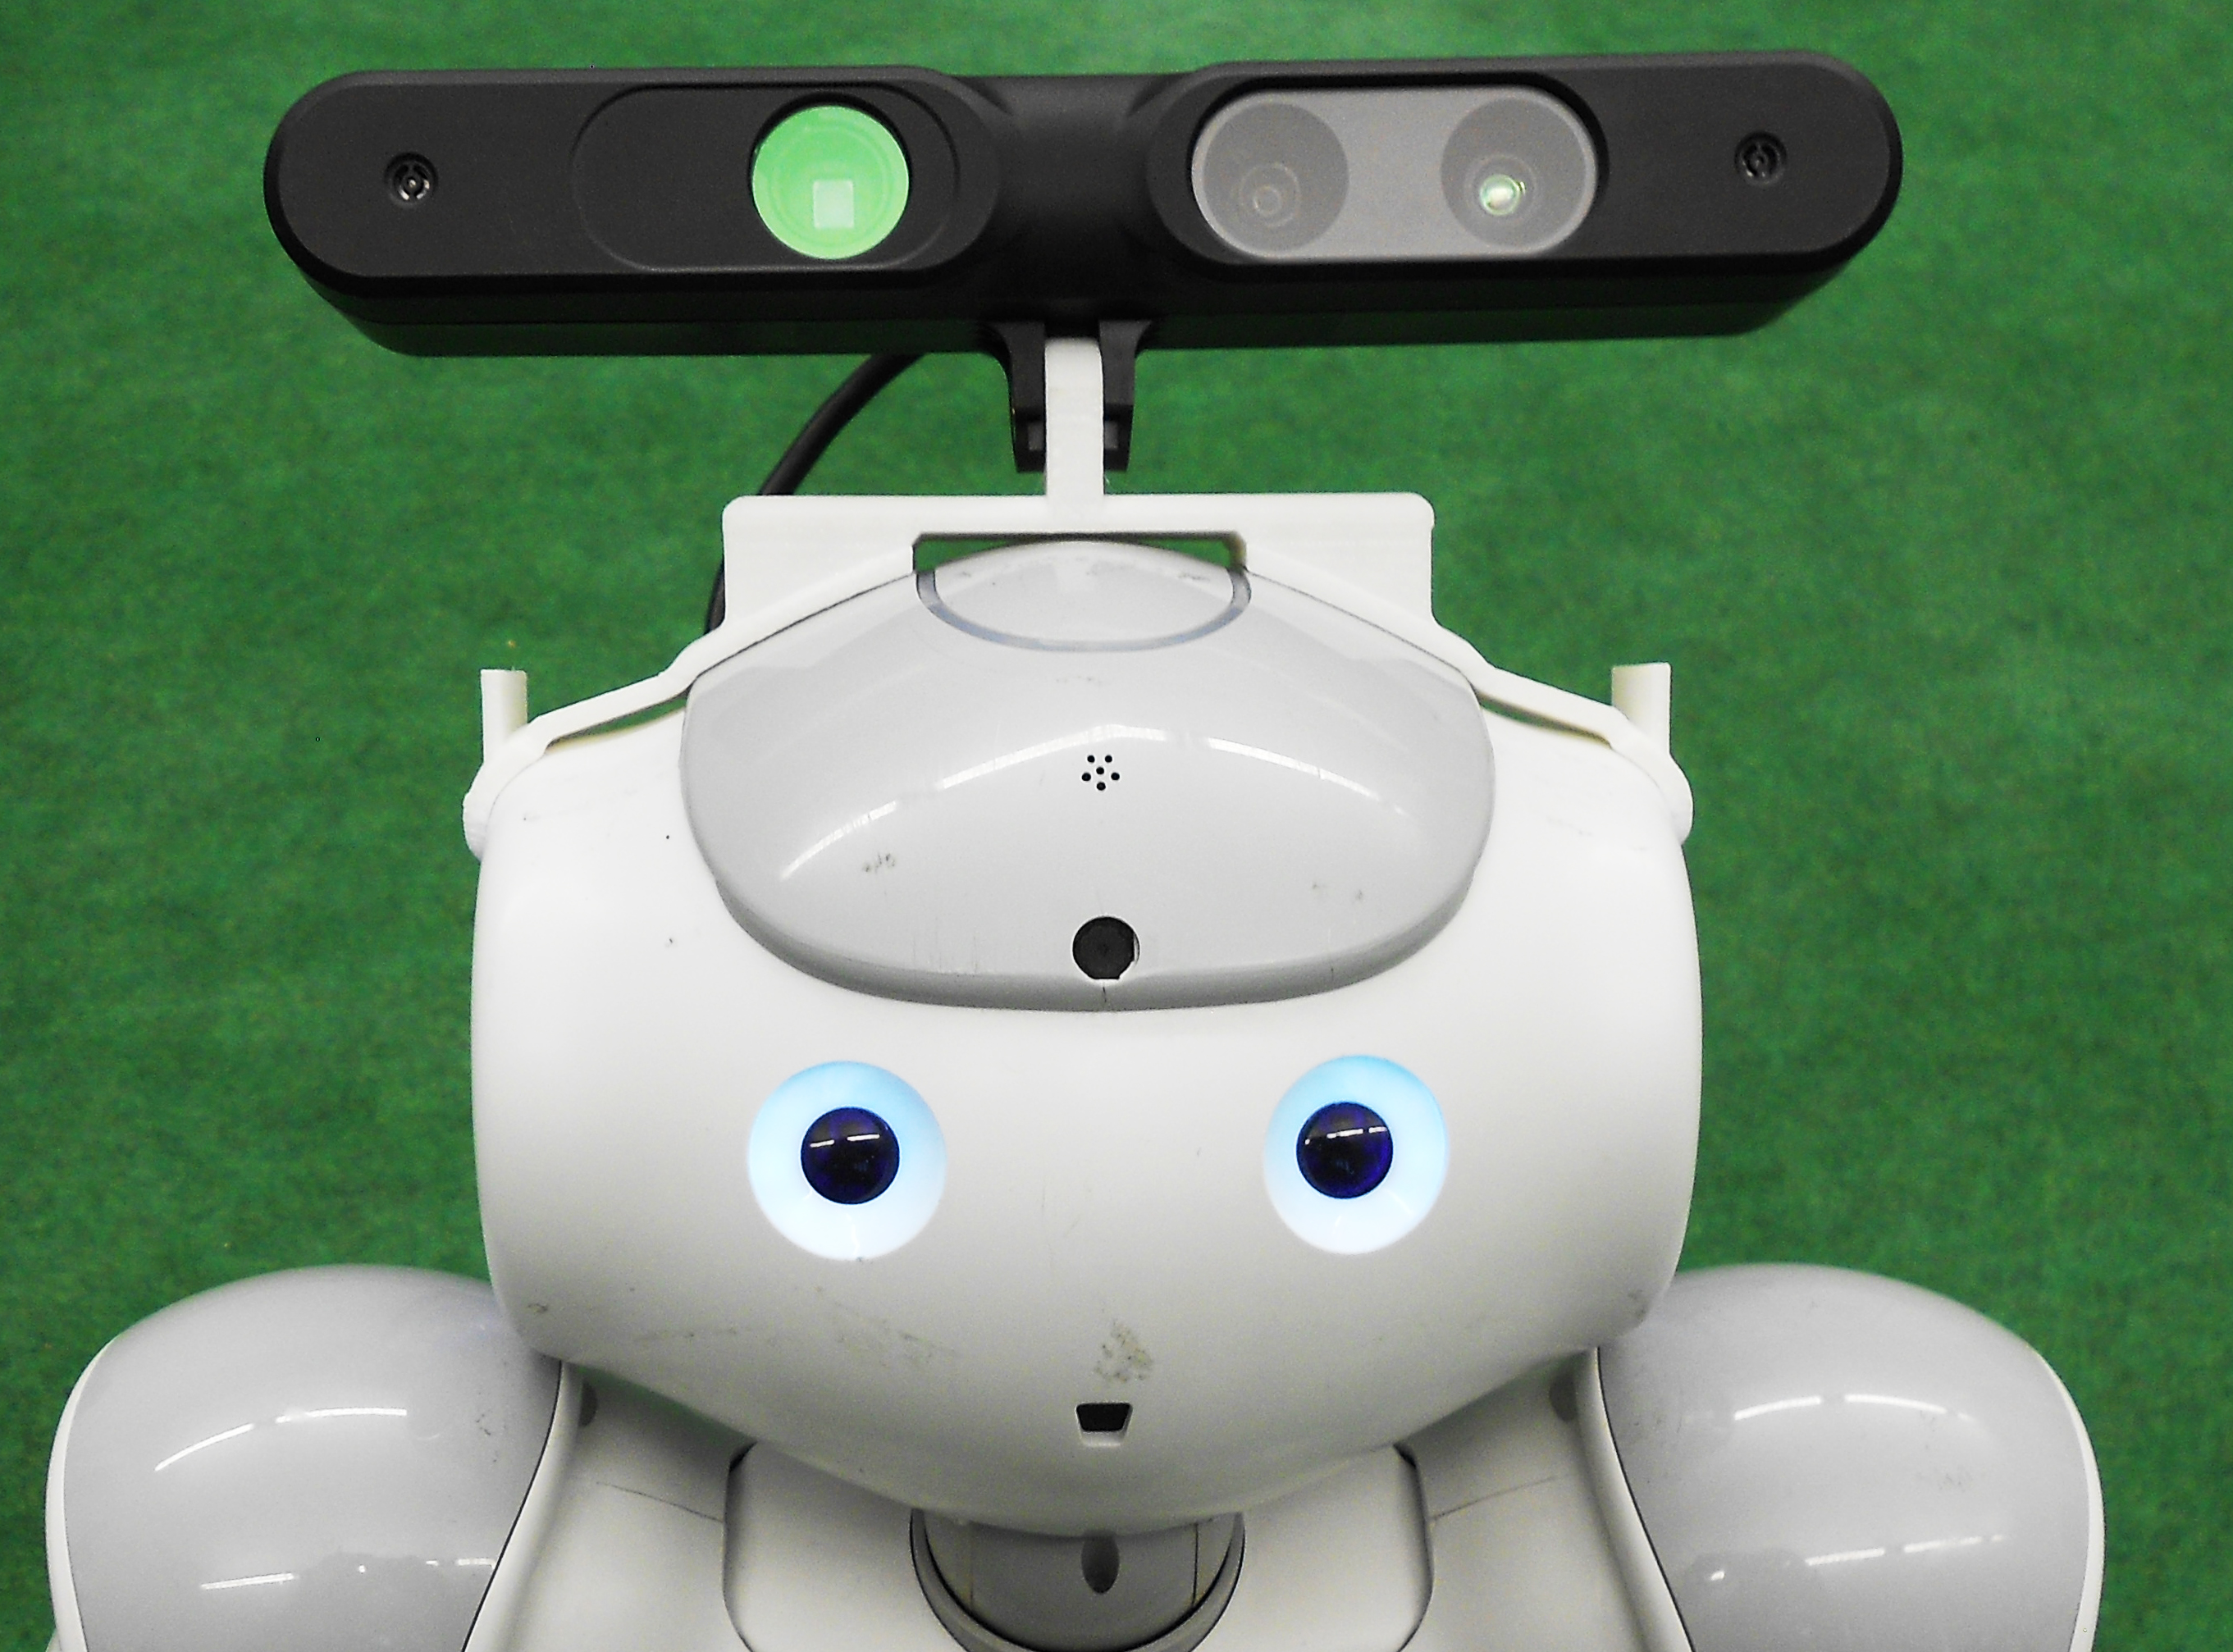
\includegraphics[height=60mm]{figures/content/xtion-mount.jpg} \caption*{Asus Xtion mounted on NAO}
	\end{minipage}
\end{figure}
\label{fg:xtion:mount}



\paragraph*{3D Printed NAO Xtion Mount} We have found a solution that is designed by emotion-robotics.com. Therefore, we have used their 3D model to print it using MakerBot Replicator 5th Generation 3D Printer as shown in the figure \ref{fg:xtion:mount}. The original base of Asus Xtion is removed and the camera is screwed with the 3D printed mount, and easily fixed on the head of the robot. 

%
%% Sections
%\section{Gesture Recognition}
Above sections described the necessary tools that are implemented to execute a real time hand gesture recognition system. In this thesis we have decided to train the system with static gestures. However, the system can be easily extended to recognize temporal gestures with the flexibility of Gesture Recognition Toolkit (GRT). Initially a set of simple gestures are chosen and the training data is collected for all those gestures.

\subsection{Hand Gestures Modeling}
In this thesis we have modeled five static hand gestures involving both the hands of the user. These are communicative hand gestures and they symbolize few referential action. Apart from Sign Language used by people with speech disability, various hand gestures are being used by humans in their day to day living. Figure \ref{fg:ges:signal} shows the hand signals used by different personnels in wide variety of application.

\begin{figure}
	[h] \centering 
	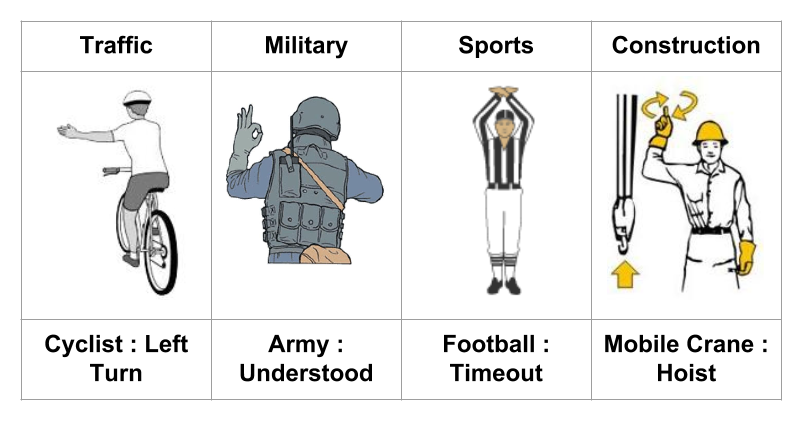
\includegraphics[height=7cm]{figures/content/ges-signals.png} \caption{Hand Signals} \label{fg:ges:signal} 
\end{figure}


This thesis focuses on hand gesture recognition to felicitate Human-Robot interactions. One greater application using hand gestures for robots is commanding the robot to move to another position. Additionally it could translate the gestures to spoken words to help people with speech disability.   

\begin{figure}
	\centering 
	\begin{minipage}
		{.45 
		\textwidth} \centering 
		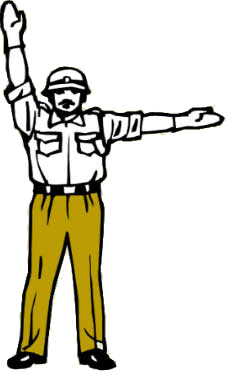
\includegraphics[height=7cm]{figures/content/ges-turn-left.jpg} \caption{Turn Left Gesture} \label{fg:ges:2} 
	\end{minipage}
	\begin{minipage}
		{.45 
		\textwidth} \centering 
		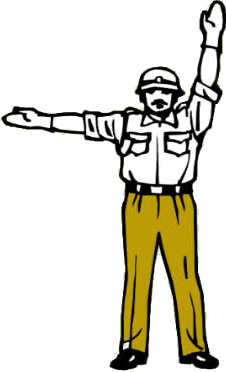
\includegraphics[height=7cm]{figures/content/ges-turn-right.jpg} \caption{Turn Right Gesture} \label{fg:ges:3} 
	\end{minipage}
	\begin{minipage}
		{.45 
		\textwidth} \centering 
		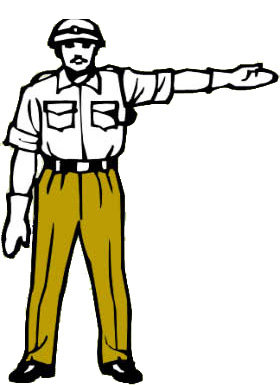
\includegraphics[height=7cm]{figures/content/ges-move-left.jpg} \caption{Move Left Gesture} \label{fg:ges:4} 
	\end{minipage}
	\begin{minipage}
		{.45 
		\textwidth} \centering 
		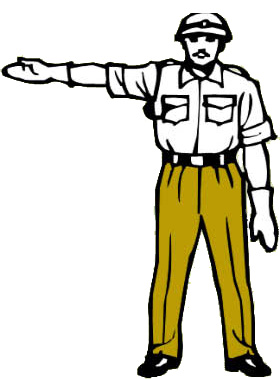
\includegraphics[height=7cm]{figures/content/ges-move-right.jpg} \caption{Move Right Gesture} \label{fg:ges:5} 
	\end{minipage}
	\begin{minipage}
		{.45 
		\textwidth} \centering 
		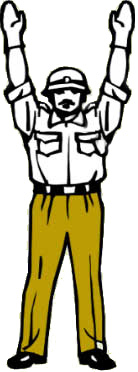
\includegraphics[height=7cm]{figures/content/ges-walk.jpg} \caption{Walk Gesture} \label{fg:ges:1} 
	\end{minipage}	
\end{figure}
\label{fg:ges:hands} 


Therefore, we have chosen five simple static gestures as shown in the figure \ref{fg:ges:hands} which are conceptualized by the traffic police hand signals. All the gestures are modeled to the direction of the user and they will be understood as mirrored gestures. For example, left side of the user will be right side to the robot that is facing the user. Additionally our system makes use of two dynamic gestures of NiTE which are used as focus gestures to gain control or start hand tracking.

\paragraph*{Turn Left} It is gesticulated as shown in the figure \ref{fg:ges:2} by holding the right hand up and left hand wide open. It refers to an action that turn to left and stay in position. 

\paragraph*{Turn Right} It is gesticulated as shown in the figure \ref{fg:ges:3} by holding the left hand up and right hand wide open. It refers to an action that turn to right and stay in position. 

\paragraph*{Move Left} It is gesticulated as shown in the figure \ref{fg:ges:4} by holding the right hand down and left hand wide open. It refers to an action that turn to left and keep moving in the forward direction.

\paragraph*{Move Right} It is gesticulated as shown in the figure \ref{fg:ges:4} by holding the left hand down and right hand wide open. It refers to an action that turn to right and keep moving in the forward direction.

\paragraph*{Walk} It is gesticulated as shown in the figure \ref{fg:ges:4} by holding the left and right hand up. It refers to an action that keep moving in the forward direction.

\paragraph*{Wave} It is gesticulated by holding a hand up and move it several times from left to right and back. This gesture is executed to initiate hand tracking, if no hands are tracked or tracked hand is been lost.

\paragraph*{Click} It is gesticulated by holding a hand up, push the hand towards the sensor then immediately pull the hand backwards. 

\subsection{Training} 
Our gesture recognition pipeline is configured to have 15 seconds preparation time and 20 seconds recording time with 6 dimensional input of both left and right hands at positions x, y and z in the Cartesian coordinates. Depth camera is at the origin of the coordinate system as shown in the figure \ref{fg:xtion:origin}.

\begin{figure}
	[h] \centering 
	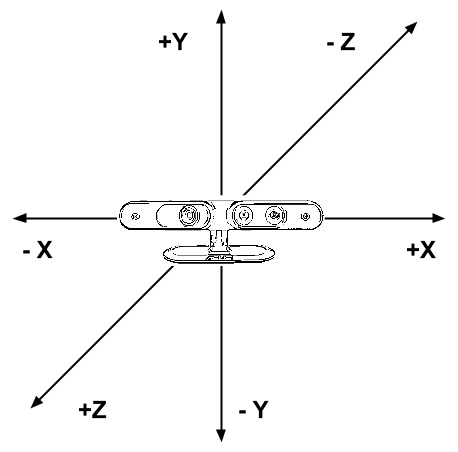
\includegraphics[height=6cm]{figures/content/xtion-origin.jpg} \caption{Depth Camera origin} \label{fg:xtion:origin} 
\end{figure}


Brain is set to training mode and CC is started to visualize the hand positions in order to align the trainer during the preparation time. Each gesture is isolated in time and gesticulated for 20 seconds. Samples are added to the training dataset and when the timer stopped the recording, Brain asked the trainer to train the same class again or another. Every gesture was assigned a class label from 1 to 5 and the mapping of class label to hand gesture is stored in a configuration file named signs.json. 

\begin{figure}
	[h] \centering 
	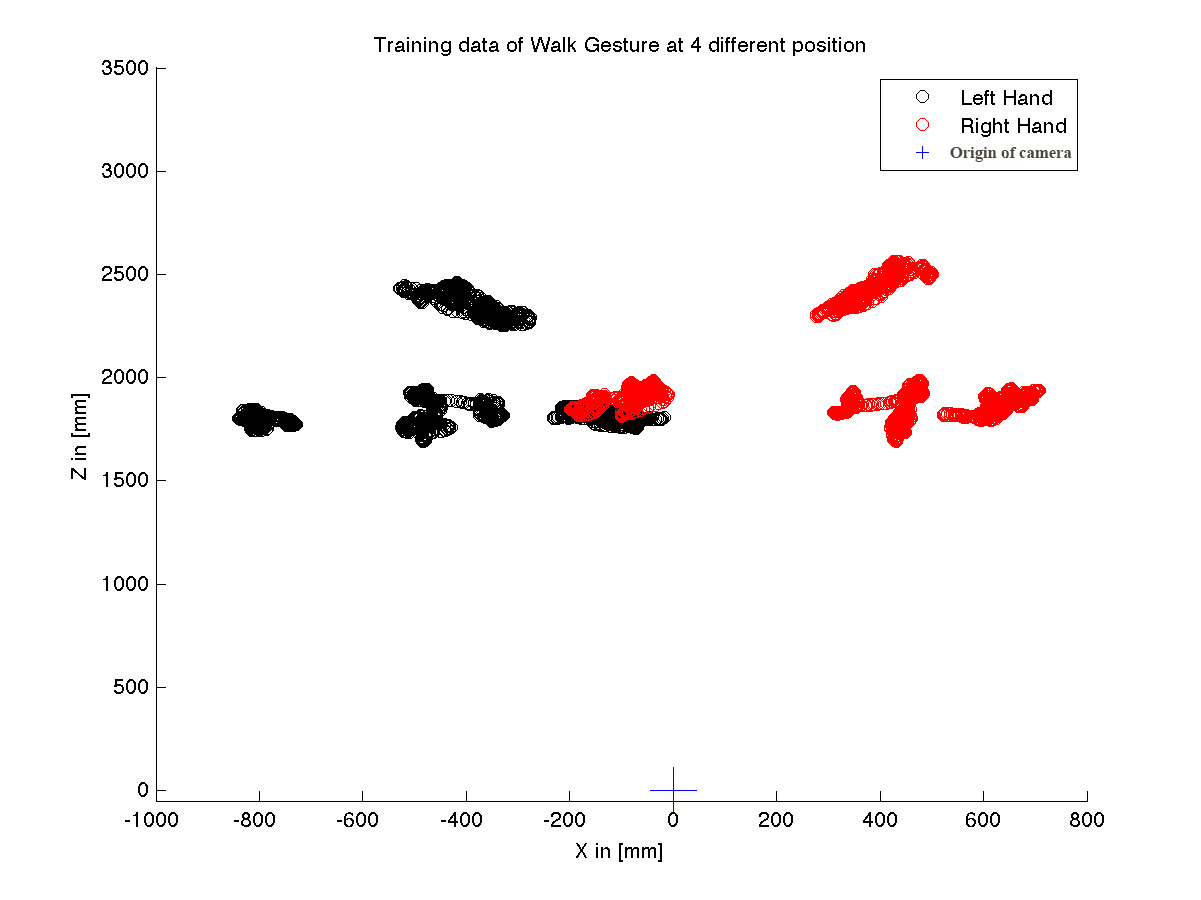
\includegraphics[height=10cm]{/result/train-walk-all.jpg} \caption{Training data of walk gesture recorded in 4 different positions with the minimum distance from 1700 mm to the maximum distance 2500 mm away from the sensor and 800 mm left or right to the origin of the depth camera.} 
	\label{fg:ges:pos} 
\end{figure}


\paragraph*{Minimum and Maximum Distance Training} \label{sec:range:train} If the gestures are gesticulated with only one person at a static position in space in front of the camera, then the recognition algorithm would not recognize the same gesture gesticulated by another person or the same person in different position. In order to scale the range of recognition, every gesture was gesticulated in 4 different positions as shown in the plot \ref{pl:ges:pos} and in all possible combinations that hands are kept wider or narrower as shown in the plots \ref{fg:ges:plot}. Therefore, each gesture in the training data is recorded in 4 positions with each for 20 seconds at 30 samples per second created 2400 samples per gesture. 

ANBC is an iterative learning algorithm that improves the classification accuracy with increase in positive training data. Plot \ref{fg:ges:plot} shows that the trained data makes our gesture recognition system to detect gestures at the minimum distance from 1700 mm to the maximum distance 2500 mm away from the sensor and 800 mm left or right to the sensor. If the user leaves this field of view, the hand tracking algorithm will lose the hand or gesture will fall in the Null Rejection region of the classifier.

\begin{figure}	 	
	\begin{minipage}
		{.45 
		\textwidth}  
		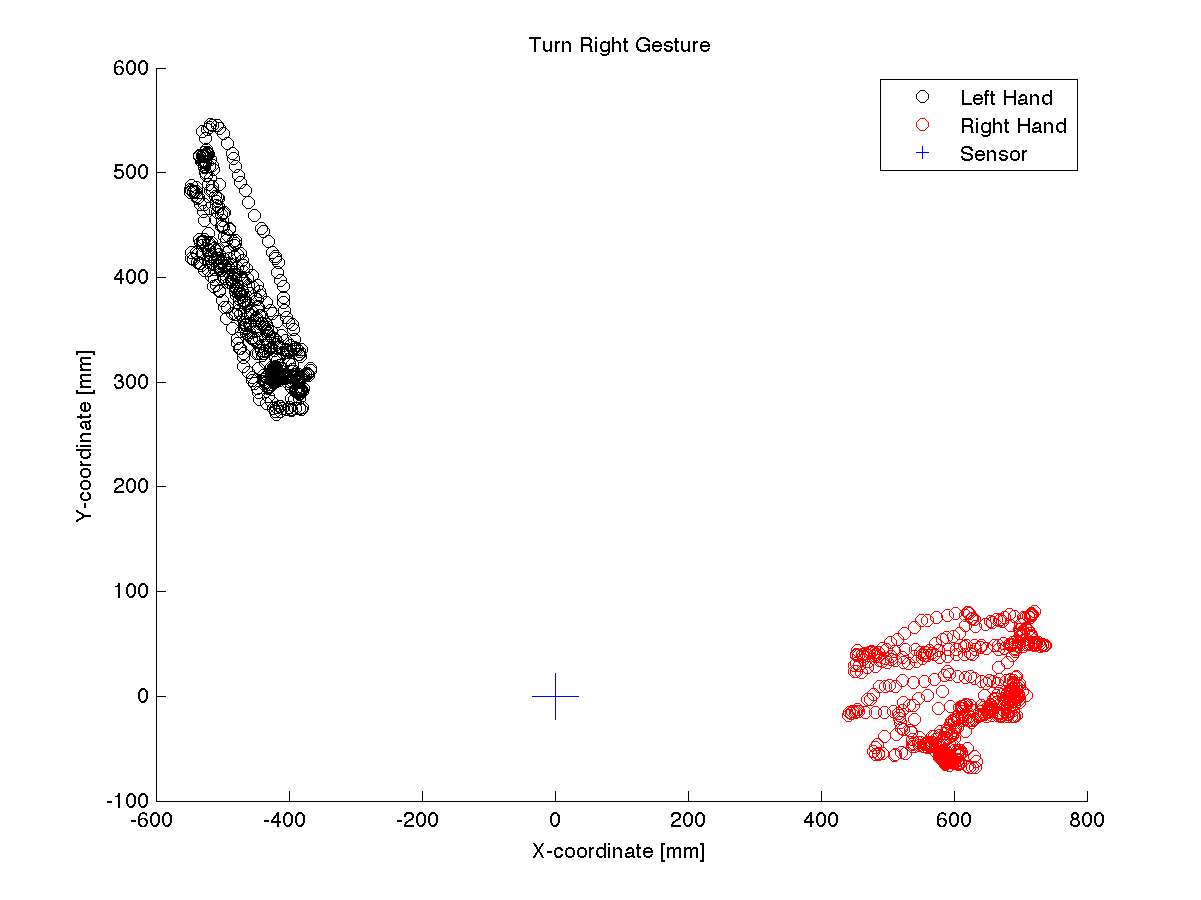
\includegraphics[height=60mm]{figures/result/plot-ges-2.png} \caption{Turn Left Gesture} \label{pl:ges:2} 
	\end{minipage}
	\begin{minipage}
		{.45 
		\textwidth}  
		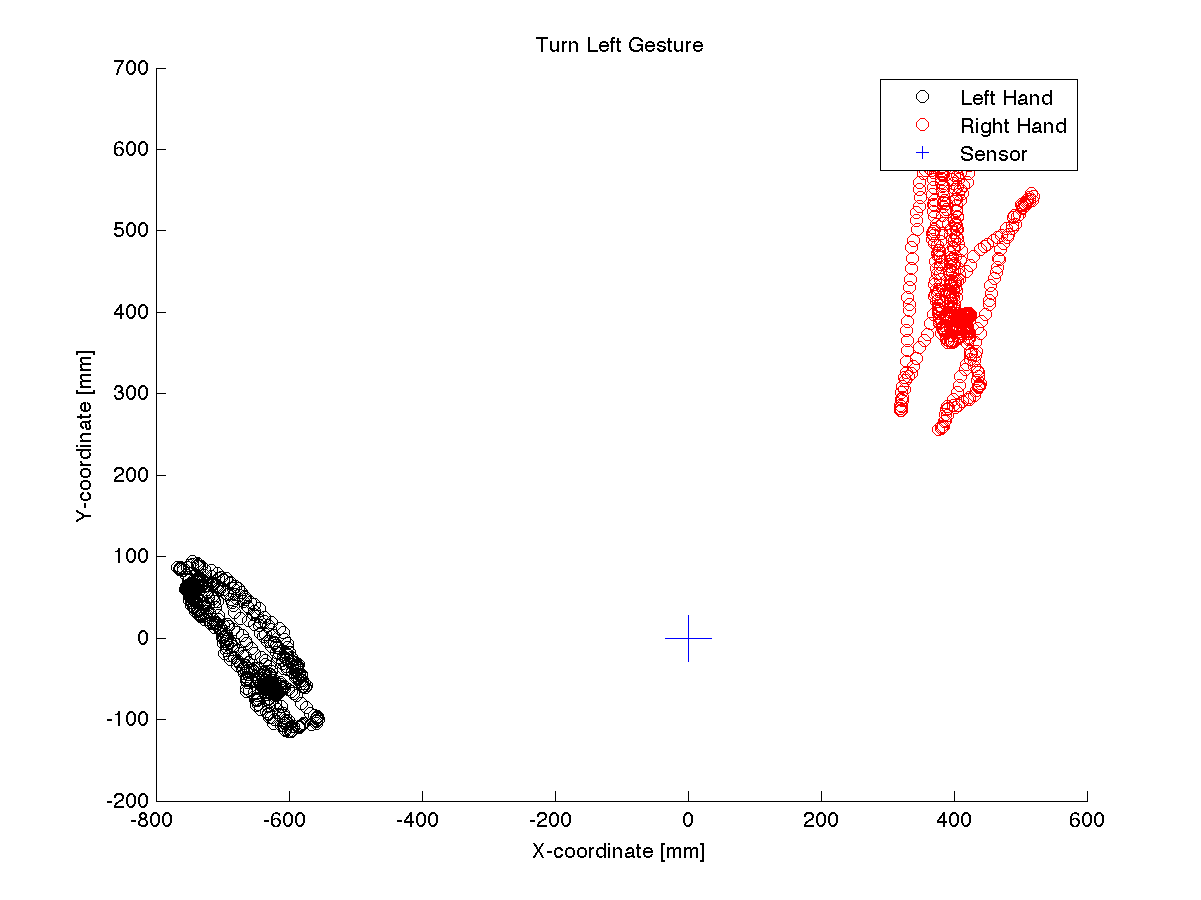
\includegraphics[height=60mm]{figures/result/plot-ges-3.png} \caption{Turn Right Gesture} \label{pl:ges:3} 
	\end{minipage}
	\begin{minipage}
		{.45 
		\textwidth}  
		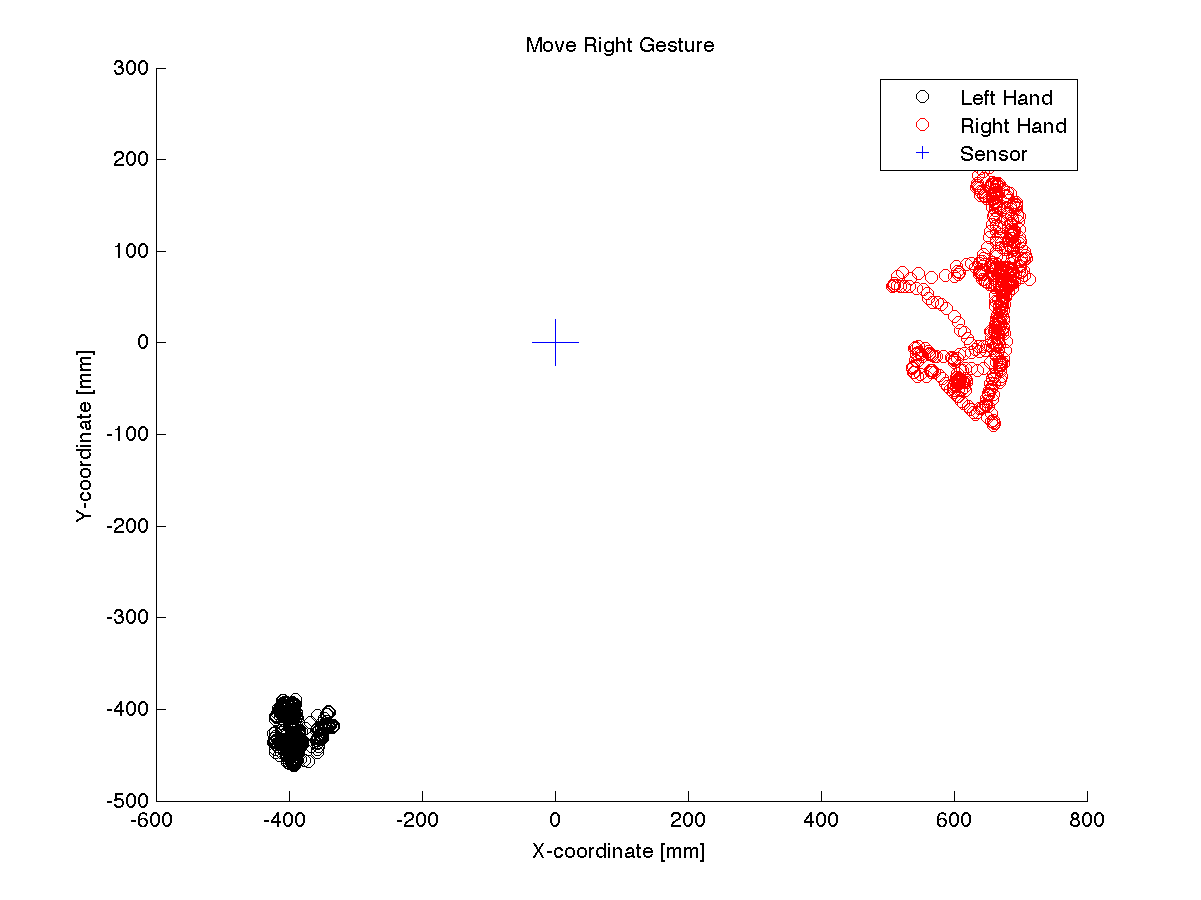
\includegraphics[height=60mm]{figures/result/plot-ges-4.png} \caption{Move Left Gesture} \label{pl:ges:4} 
	\end{minipage}
	\begin{minipage}
		{.45 
		\textwidth}  
		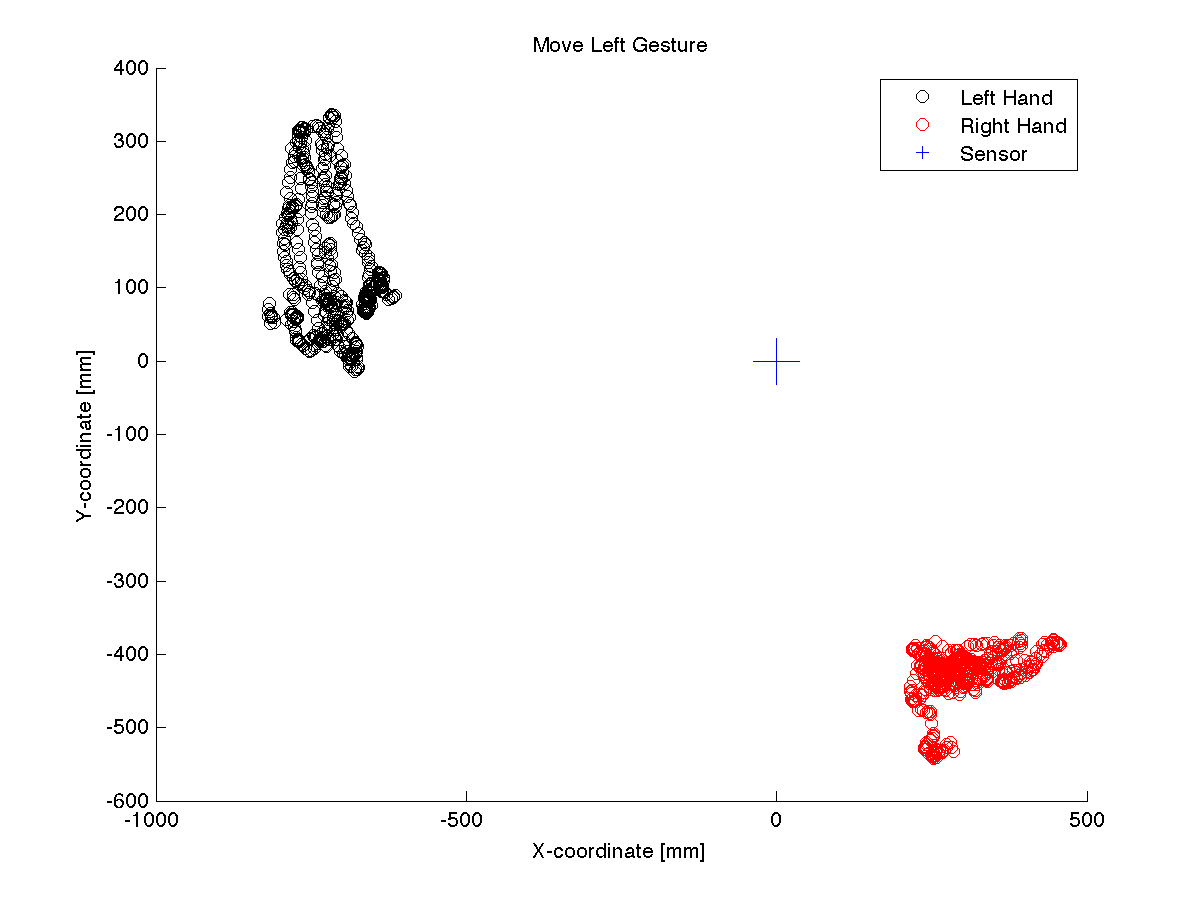
\includegraphics[height=60mm]{figures/result/plot-ges-5.png} \caption{Move Right Gesture} \label{pl:ges:5} 
	\end{minipage}
	\begin{minipage}
		{.45 
		\textwidth}  
		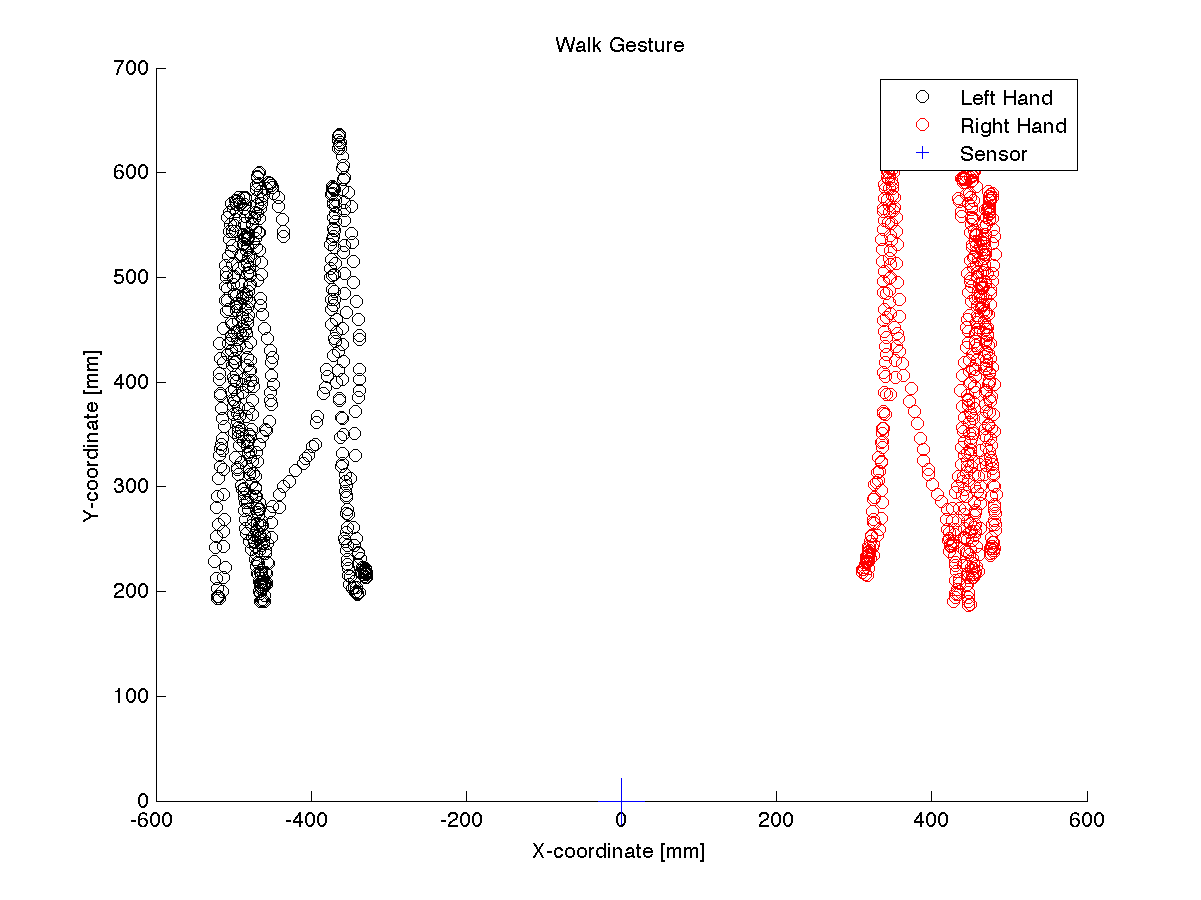
\includegraphics[height=60mm]{figures/result/plot-ges-1.png} \caption{Walk Gesture} \label{pl:ges:1} 
	\end{minipage}	
\end{figure}
\label{fg:ges:hands} \label{fg:ges:plot}



\paragraph*{Training Data} Once all the gestures are recorded, they replayed using CC to find out, if there is any false samples are added to the training data. Such false data leads to an incorrect model that will ultimately affect the prediction performance. Such samples are removed from the training data and a final dataset with all 5 classes are stored as hri-training-dataset.txt. Additionally, some test data for each gesture is recorded in order to evaluation the accuracy of the recognition system. Furthermore, a set of non-gesture dataset was recorded in order to test the Null Rejection accuracy of the classifier. 

\subsection{Prediction} After successfully collecting the training data for all the gestures, Brain is set to prediction mode where the pipeline is trained. HRI module starts to track the user's hand, Brain predicts a gesture when both the hands are present in the input sample. Figure \ref{fg:cc:ges:1} shows Control Center where prediction output for every sample with maximum likelihood is displayed all the time. The predicted gesture is triggered only after it was gesticulated for more than one second.

\begin{figure}
	[h] \centering 
	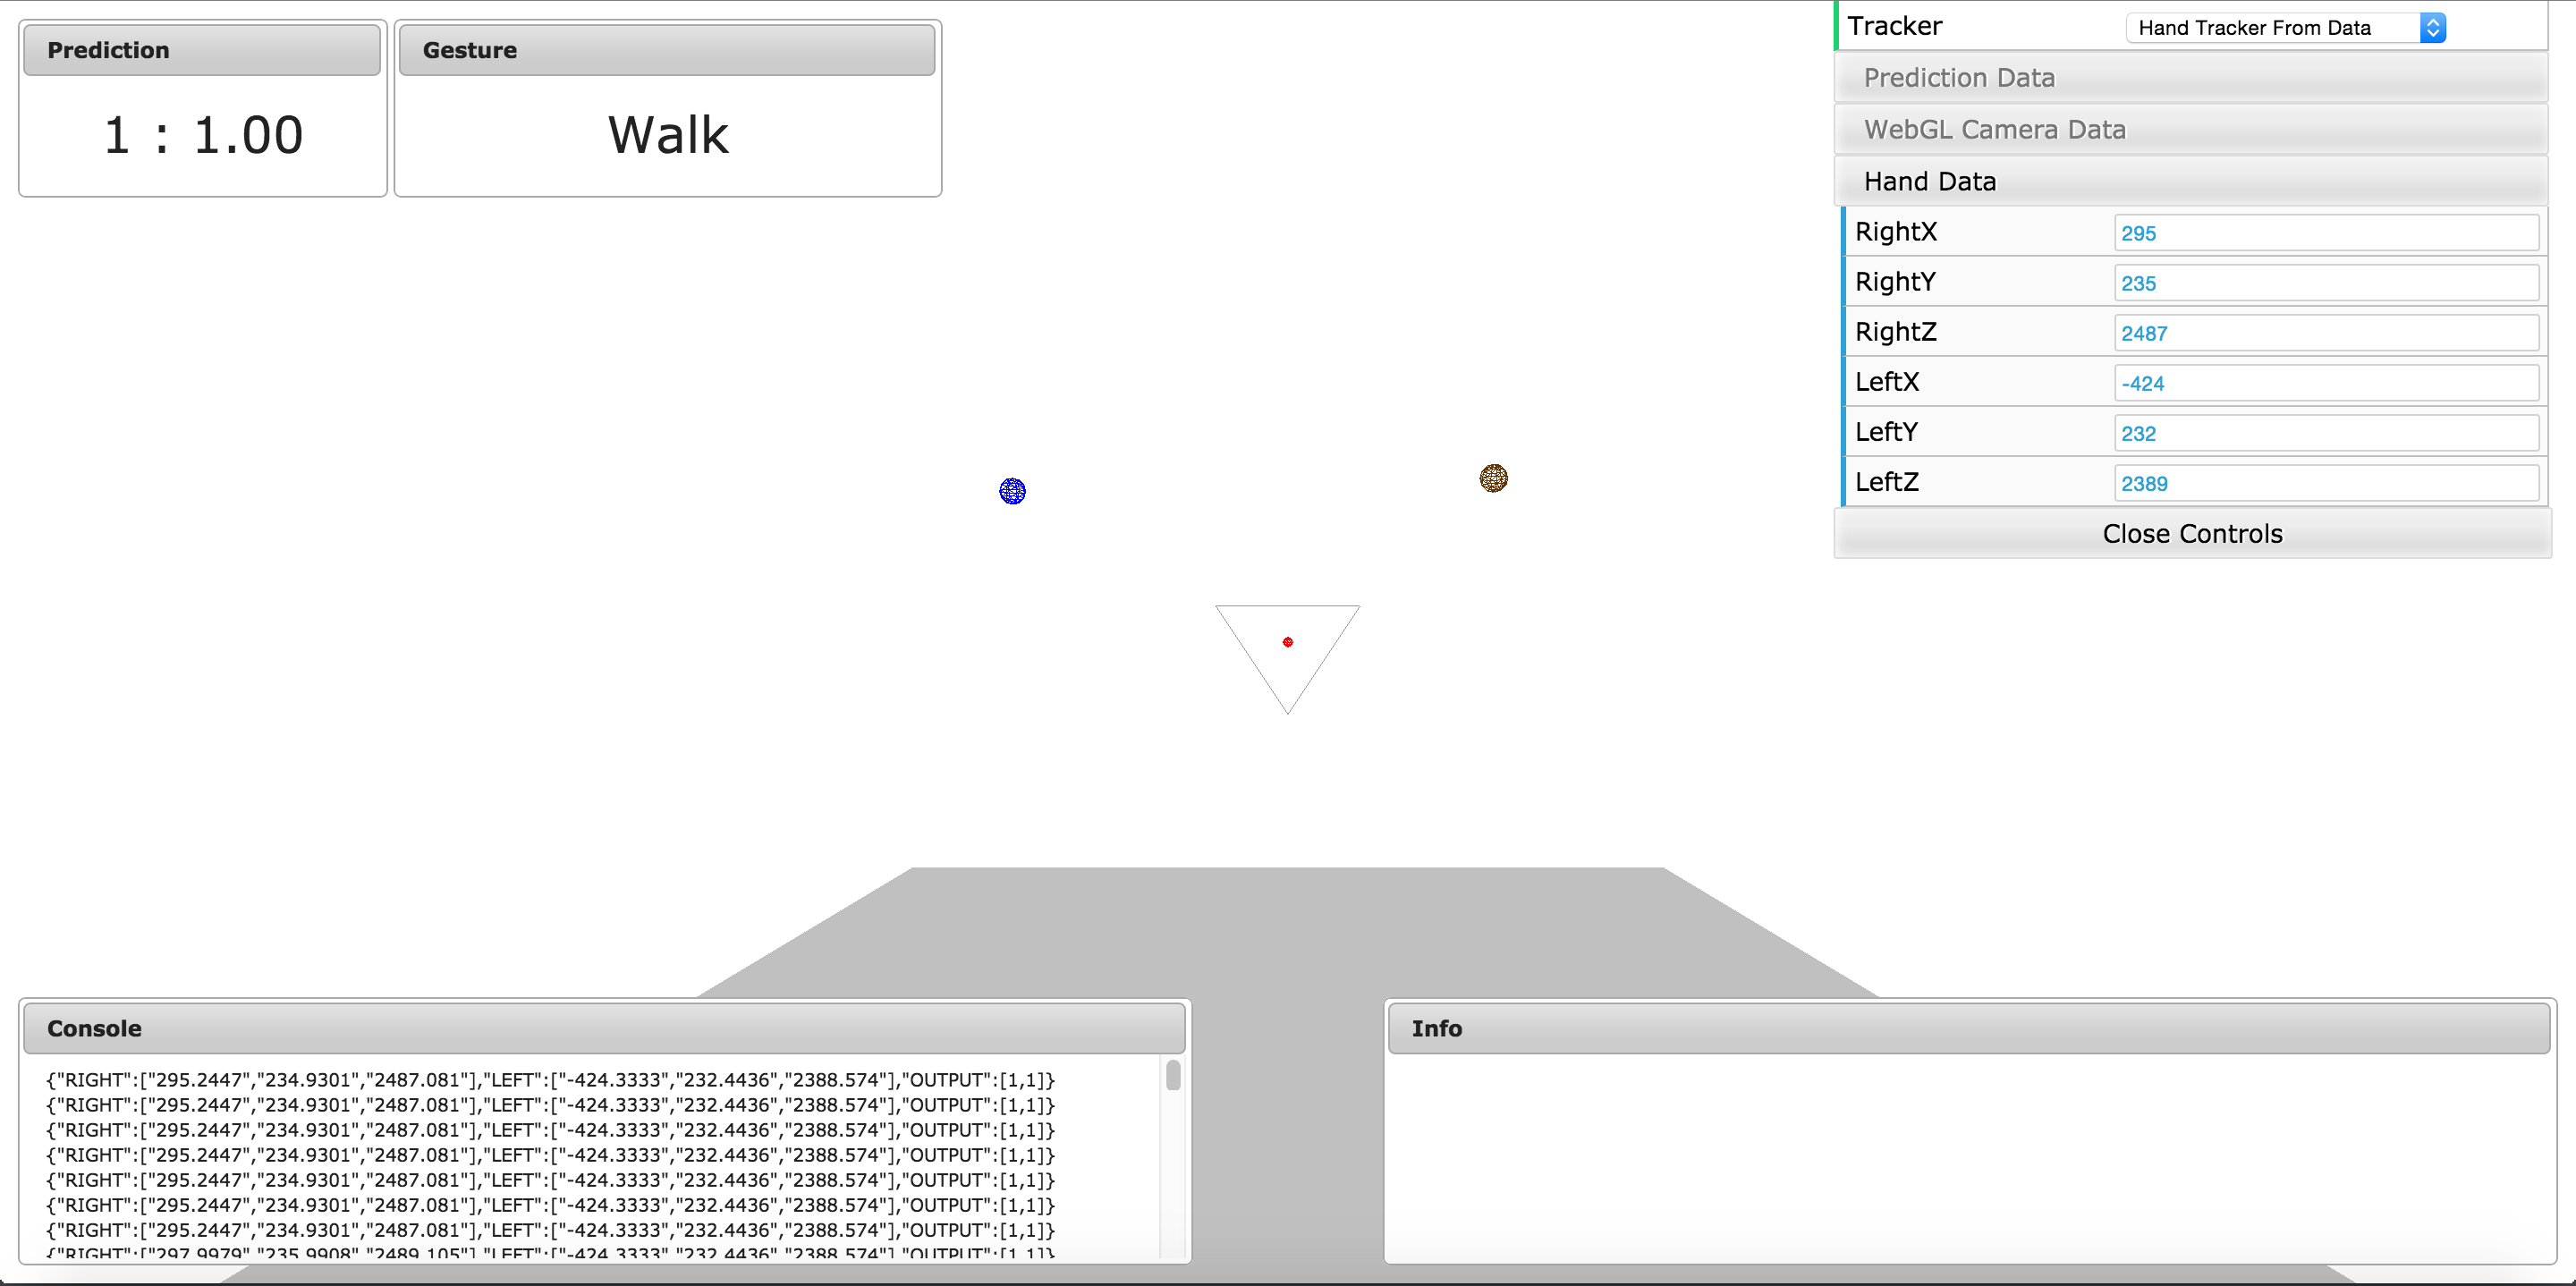
\includegraphics[height=7cm]{figures/result/cc-ges-1.png} \caption{Walk Gesture} \label{fg:cc:ges:1} 
\end{figure}


%\section{Human-Robot Interaction} Fundamental goal of this thesis to build a systematic hand gesture recognition system to interact with machines such as robot or a computer. Interaction with them are mostly through displays, keyboards, mouse and touch interfaces. These devices have grown to be familiar but inherently limit the speed and naturalness. Previous sections have explained how we have built a system to facilitate a natural interaction with the humanoid robot called NAO. Following sections illustrate how robot reacts to the hand gestures in real time with the help of Command module.

\subsection{Gesture-to-Speech} Easiest translation from the recognized hand gesture is to speak it out loud. We have used Text-To-Speech (TTS) engine that is built internally inside Aldebaran modules. When the user gesticulate the focus gesture, NAO says "WAVE" and denoting that hand tracking is started. Furthermore, the robot says words such as "Walk", "Turn Left", "Turn Right", "Move Left" and "Move Right", whenever those gestures are recognized. Additionally, it says info messages such as "Left Hand is lost", "Right Hand is lost" and "Both hands are lost" to inform the user about the internal status of hand tracking.

\subsection{Gesture-to-Motion} This thesis is initially conceived as a hand gesture translator just to say the recognized gestures loud. To make this system more useful, Gesture-to-Motion feature is added to the Command module. This functionality helps us to move the robot from one position to another in 2 dimensional space. Therefore each gesture is assigned a locomotion task as follows:

\paragraph*{Walk} This gesture commands the robot to walk in forward direction at a normalized maximum velocity (1.0) with the step frequency of 0.5. Robot walks approximately for 5 seconds and waits for the next command.

\paragraph*{Turn Left} This gesture commands the robot to rotate itself around z-axis in the left direction at a normalized maximum velocity (1.0) with the step frequency of 0.5. Robot walks approximately for 3 seconds and waits for the next command.

\paragraph*{Turn Right} This gesture commands the robot to rotate itself around z-axis in the right direction at a normalized maximum velocity (1.0) with the step frequency of 0.5. Robot walks approximately for 3 seconds and waits for the next command.

\paragraph*{Move Left} This gestures combines Walk and Turn Left by commanding the robot to rotate itself around z-axis in the left direction for 3 seconds and walk forward for 5 seconds and waits for the next command.

\paragraph*{Move Right} This gestures combines Walk and Turn Right by commanding the robot to rotate itself around z-axis in the right direction for 3 seconds and walk forward for 5 seconds and waits for the next command.

\paragraph*{Click} This gesture is used to gain the control of the robot, when the robot lost its balance and is fallen down. When this gesture is executed, robot wakes up from the sleeping mode and sets itself to the standing position.

\begin{figure}	 	
	\begin{minipage}
		{.6
		\textwidth}  	
		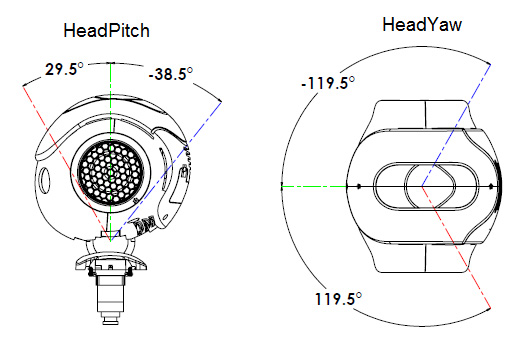
\includegraphics[height=60mm]{figures/content/nao-head.jpg} \caption{NAOs head Pitch and Yaw angle range that can be set with the help of joint control methods of NAOqi API. \cite{8} } \label{fg:nao:head} 
	\end{minipage}
	\hspace{10 mm}
	\begin{minipage}
		{.3
		\textwidth}  
		\centering
		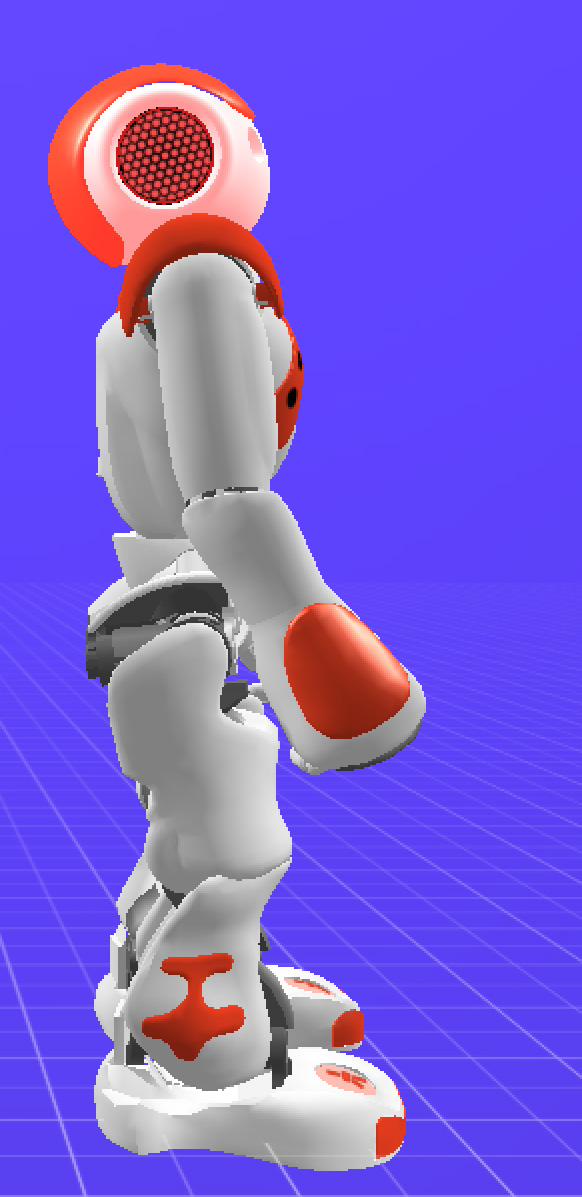
\includegraphics[height=70mm]{figures/content/nao-head-stand.jpg} \caption{Virtual NAO in Aldebaran Choregraphe with head pitch set to -18 degrees look at the upper body of the user.} \label{fg:nao:head:stand} 
	\end{minipage}	
\end{figure}




\subsubsection*{Head Position} As described in the section \ref{sec:range:train}, collection of training data for each gesture is carried out in 4 different positions in front of the robot. During this phase robot is set to standing position where the height of the robot is 58 cm. Figure \ref{fg:nao:head} shows that NAOs head can be tilted by adjusting the pitch and yaw of the head joint. In order to avoid confusing camera perspective during the training, NAOs head pitch is set to -18.0 degrees and yaw is set to 0.0 degree as shown in the figure \ref{fg:nao:head:stand}. At this angle, field of view of the depth camera is enough to cover upper body of the user. 

However, keeping the head tilted with mounted camera will cause the robot to lose balance. Therefore, NAOs head position is reset to initial stand position before it executes the received Gesture-to-Motion command. Once the locomotion phase is completed, it looks back at the user. This functionality greatly improves in locating the user at any position in the Minimum-Maximum range as show in the plot \ref{pl:ges:pos}.

\subsection{Gesture-to-Gesture} Apart from offering the essential functionalities, Command module also provides Gesture-to-Gesture translation where NAO will be imitating hand gestures of the user. Shoulder Roll and Pitch, Shoulder Roll and Yaw angles are measured by manually by positioning NAO for every gesture. When a gesture is detected, the Command modules sets the predefined angles to the shoulder and elbow joints of both the hands of NAO, therefore, translating the human hand gesture to a robotic hand gesture.

%\section{Toolchain} During the implementation of this thesis, many tools are used for various purposes. Every module in this thesis uses different programming language, therefore, different toolchains are used. Following sections talk about the tools that are used to develop, build, deploy and document this thesis work. 

\subsection{Develop}
\paragraph*{Xcode} Core functionalities of this thesis are developed in C++ on Mac OSX. Therefore, Xcode is used to develop HRI and Brain module. Xcode is an IDE containing a suite of software development tools developed by Apple for developing software for OS X and iOS.

\paragraph*{WebStorm} Control Center module is developed in Javascript with the help of a popular IDE for Web development called as WebStorm. It is a commercial IDE for JavaScript, CSS and HTML built on JetBrains IntelliJ IDEA platform.

\paragraph*{PyCharm} Command module is developed in Python using an IDE name as PyCharm. It is implemented by a company called JetBrains and it provides code analysis, a graphical debugger, an integrated unit tester and supports web development with Django.

\subsection{Build}
\paragraph*{Javascript and Python} They are traditionally implemented as interpreted languages and therefore they do not need any special compilers to build them. Control Center module needs just a latest browser with WebSocket and WebGL support to run the Javascript code. Python binary is available is most modern operating systems and we used Python version 2.7.6 to run Command module. 

\paragraph*{C++} The code that was implemented in C++ used 2 different compilers to build it, because the development is done on 64-bit Mac operating system and target system is a 32-bit Gentoo Linux operating system. 

\paragraph*{\indent Clang and Xcode} Development code was built using Clang with LLVM libc++ Standard library. Clang is a compiler developed by Apple for C, C++, Objective-C and Objective-C++ programming languages. Build settings such as header, library search paths, macros, environment variables and linking are configured using Xcode. 

\paragraph*{\indent GCC and Cmake} Production code was built using GNU Compiler Collection (GCC) with libstdc++ GNU++11 Standard library. It is a compiler system produced by the GNU Project supporting various programming languages such as C, C++, Objective-C, Objective-C++, Fortran, Java, Ada, and Go.  Build settings such as header, library search paths, macros, environment variables and linking are configured using Cmake. CMake is cross-platform free and open-source software for managing the build process of software using a compiler-independent method. 

The repository is cloned on OpenNAO and then HRI module was built as shown in \ref{code:build} and then the executable is copied to NAO OS. However, a patch as described in the section \ref{sec:patch} must be applied on OpenNAO and NAO OS in order to build the sources.

\lstinputlisting[language=python]{code/build.sh} \label{code:build}

\subsection{Patch} \label{sec:patch}
\paragraph*{OpenNAO / NAO OS} Aldebaran provides an image of the NAOs operating system named as OpenNAO to use the robotic system virtually and it can run in a virtual machine in any host. OpenNAO is 32-bit Gentoo Linux modified by Aldebaran for Intel Atom Processor with i686 Architecture. 

\paragraph*{Emerge} Emerge is the package manager for Gentoo Linux and Portage is the package tree.  Aldebaran forces users not to update Emerge to avoid conflict with Aldebaran modules. Portage tree used with NAO OS was last updated on 11 Jan 2012. 

\paragraph*{GCC 4.5.3} Due to outdated packages on OpenNAO, GCC version is 4.5.3 and C++ library version is libstdc++.so.6.0.14. NiTE middleware library (libNiTE2.so) was built by PrimeSense using higher version of GCC (higher than GLIBCXX\_3.4.14 or libstdc++.so.6.0.14). Therefore, building HRI module on OpenNAO will throw an error while linking libNiTE2.so, '/usr/lib/libstdc++.so.6: version GLIBCXX\_3.4.15 not found'

This issue was solved by finding higher version of libstdc++ from debian repository for 32-bit architecture and copying that to /usr/lib folder on OpenNAO/NAO OS and linking current libstdc++ to the copied version. Repository of our thesis contains the required version of libstdc++. Following shell commands show how it must be patched on OpenNAO or NAO OS to run HRI module without any errors.

\lstinputlisting[language=python]{code/gcc-patch.sh}

\subsection{Version Control} Proposal to final results of a project goes through many iterations or modification of the source files. Such changes are intentional and sometimes they are accidental. Therefore, source files of this thesis are stored and tracked using a version control system called Git. Git is a version control is a system that records changes to a file or set of files over time. To avoid accidental lose of source files, free git online service such as GitHub allows us to store them in a remote repository that can be cloned from anywhere via Internet. \url{https://github.com/AravinthPanch/gesture-recognition-for-human-robot-interaction} is the link to the online repository that contains all the informations regarding this thesis.

\subsection{Data Analysis} During this thesis work, significant amount of data are collected. These data consist of training and test data of full body skeletal points / hand joints which are recorded to train and test the hand gesture recognition system. This information mus be analyzed and studied for the purpose of statistically understand this system. Additionally, these data must be plotted as shown in the graph \ref{fg:ges:plot} and hence, MATLAB is used. MATLAB is a multi-paradigm numerical computing environment developed by MathWorks to do matrix manipulations, plotting of functions and data and implementation of algorithms. 

\subsection{Documentation} Proper documentation is a crucial part of any research work. Therefore, we have used LaTeX to document this thesis. LaTeX is a high-quality typesetting system that includes features designed for the production of technical and scientific documentation. TeXstudio on Mac OSX is the editor that was used to compose and manage the LaTeX documents of this. LaTeX source files can be found inside the document folder of the git repository of this thesis.
